% 九州工業大学 情報工学部 情報・通信工学科
% 卒業論文
% LaTeXテンプレートファイル

%%%%%%%%%%%%%%%%%%%%%%%%%%%%%%%%%%%%%%%%%%%%%%%%%%%%%%%%%%%%%%%%%%%%%%%%%%%%%%%%
% ・両面印刷用のスタイルです。
%
% ・章の始まりは奇数ページになるように調整されていますが、奇数ページにならない
%  場合があります。このときは、印刷時に注意してください。
%%%%%%%%%%%%%%%%%%%%%%%%%%%%%%%%%%%%%%%%%%%%%%%%%%%%%%%%%%%%%%%%%%%%%%%%%%%%%%%%

\documentclass[12pt]{jreport}
\usepackage[dvipdfmx]{graphicx}
\usepackage{float}
% \usepackage{algorithmic}	% 擬似コードを書くため
% \usepackage{midpage}
% % スタイルファイル
% \usepackage{CSNthesis}
\usepackage{CSNthesis}
\usepackage{url}


% ページスタイルの変更 
\Name{オンコン マハルク ラフマン} % 氏名を記入
\Year{2023}        % 年度を記入

% タイトルを記入
\Title{テクニカル指標の組み合わせによる\\トレーディングアルゴリズムの提案}

% 指導教員の氏名
\Supervisor{藤原 暁宏}
%------------------------- 各人の情報 end ------------------

\begin{document}
\makeCoverPage  % 表紙

\begin{abstract}  % 文字だけの概要.〜600字程度.
  近年,金融分野で数学や情報科学を応用したフィナンシャルテクノロジーが注目を浴びている.
  その中でも,株取引においては,アルゴリズムを用いて自動的に注文を判断し実行するアルゴリズム取引が活発に行われている.
  
  このアルゴリズム取引においては,ゴールデンクロス・デッドクロスやMACDなどのテクニカル指標を用いた取引が多く用いられており,
  利益やリスクの少なさの点でも優れているとされている.また,損切りや防衛損切り,利益確
  定を行うことで最終利益が向上する傾向があることも一般的に知られている.

  本研究では複数のテクニカル指標を組み合わせたアルゴリズムを提案するとともに,トレーディングツールを用いて検証し,
  テクニカル指標の有効な組み合わせを検証することを目指す.テクニカル指標はMACD,ボリンジャーバンド,60日移動平均線,日経平均株価の4つを用いて,MACDとボリンジャーバンドを主体に既存も含めて13通りのアルゴリズムを提案する.
  
  また,提案アルゴリズムについては実際の東証の株価データを用いたバックテストを通じて,有効性の検証を行う.検証結果より,4つの提案したアルゴリズムにより,10年間の期間において100%を超える利益が得られることを示す.

\vfill\end{abstract}

\newpage
\pagestyle{plain}       % ここからページ番号表示
% 目次
\pagenumbering{roman}	% 目次のページ番号(ローマ字)
\tableofcontents 		% 目次作成
\newpage
\pagenumbering{arabic} 	% 本編ページ番号
%%%%%%%%%%%%%%%%%%%%%%%%%%%%%%%%%%%%%%%%%%%%%%%%%%%%%%%%%%%%%%%%%%%%%%%%%%%%%%%



%%%%%%%%%%%%%%%%%%%%%%%%%%%%%%%%%%%%%%%%%%%%%%
%%%%%%%%%% ここから修正して下さい。 %%%%%%%%%%
% 本文(章単位で別のファイルにして下さい。)
\chapter{はじめに}
\label{chapter:Introduction}

% ページ番号を1にする
\setcounter{page}{1}
\pagenumbering{arabic}

%%%%%%%%%%%%%%%%%%%%%%%%%%%%%%%%%%%%%%%%%%%%%%%%%%%%%%%%%%%%%%%%%%%%%%%%%%%%%%%



近年,金融分野に対して数学や情報科学を活用したファイナンシャルテクノロジーが注目を
集めている.このファイナンシャルテクノロジーの一分野として,資産運用の一つである株取引
に対して,あらかじめ定めておいた手順に従い自動的に注文の数量やタイミングを判断して取
引を実行するアルゴリズム取引が盛んに行われている.また,様々なトレーディングアルゴリズ
ムを過去のビッグデータを用いて検証可能なトレーディングツールも多数提案されている.

%%%%%%%%%%%%%%%%%%%%%%%%%%%%%%%%%%%%%%%%%%%%%%%%%%%%%%%%%%%%%%%%%%%%%%%%%%%%%%%
このトレーディングアルゴリズムに対するこれまでの研究例として,森本の研究\cite{morimoto}がある.森本は該当研究において,
一定期間における安値の最低値を計算し,その変動を折れ線グラフ
で表現したLow グラフと.一定期間における高値の最高値を計算し,そ
の変動を折れ線グラフで表現したHigh グラフに着目し,売買タイミングを
判断するアルゴリズムの考察と提案をしている.該当研究では考察・提案
した複数のアルゴリズムで既存の取引手法である,ゴールデンクロス・デッドクロスを用いたアル
ゴリズムが最終利益,リスクの少なさの点で最も優れることを示している.また,損切りや防衛損切り,
利益確定を行うことで最終利益が向上する傾向があることも示されている.

% 本研究では,過去の株式チャートを使用して,移動平均線乖離率,ゴールデンク
% ロス・デッドクロスという既存アルゴリズムの検証と,新しくLow グラフ・High グ
% ラフを使用するアルゴリズムの提案を行った.また利益最大化手法として,既存の
% 損切り・利益確定の効果検証と,それらを補う「防衛損切り」の提案を行った.実
% 験結果より既存の取引手法である,ゴールデンクロス・デッドクロスを用いたアル
% ゴリズムが最終利益,リスクの少なさの点で最も優れることが判明した.また,ア
% ルゴリズムごとに適切なパラメータは異なるものの,損切りや防衛損切り,利益確
% 定を行うことで最終利益が向上する傾向があることがわかった.
% 今後の課題として,各アルゴリズムにおいてより良い結果が得られるパラメータ
% の調査と,サンプルとなる株式銘柄数を上昇させることが挙げられる.

% 岩永は該当研究において,株式の売買期間を数日から数週間程度の比較
% 的短期間に設定する手法である「スイングトレード」に着目し,売買タイミングを
% 判断するアルゴリズムの考察と提案を行っている.なお,該当研究では考察・提案
% した複数のアルゴリズムのうち,5 日移動平均線と25 日移動平均線による「ゴール
% デンクロス・デッドクロス」のアルゴリズムにおいて最良の結果が得られている.


本研究では,様々なテクニカル指標を組み合わせて有効なトレーディングアルゴリズムの提案を目標とする.また,提案アルゴリズムについては,トレーディングツールを用いて有効性の検証を行う.
用いる指標はMACD,ボリンジャーバンド,60 日移動平均線,日経平均株価の4つであり,MACD とボリンジャーバンドを主体に既存アルゴリズムも含めて 13 通りのアルゴリズムを提案する.

また,提案アルゴリズムは,株価データに対してバックテストを行うためのツールの一つである backtesting.py を用いて実装するとともに,
実際の東証の上位の株価データに対する適用を行い,提案アルゴリズムの有効性の検証を行う.検証結果より,既存の2つのアルゴリズムと,4つの提案したアルゴリズムにより,10年間の期間において100%を超える利益が得られることを示す.また,利益,取引数は低いが平均勝率が約67%となる提案アルゴリズムも示す.

本論文は, 以下のように構築される. 第2章では, Python 言語の概要,本研究で使用した Python 言語のライブラリ,及び, 
株の基本知識と株取引で使われているテクニカル分析の指標ついて説明する.
第3章では, 本研究のテーマであるPython言語を用いたトレーディングアルゴリズムについて述べる. 第4章では, アルゴリズムの実行結果について述べる. 第5章では, 本研究のまとめを行い今後の課題について言及する.


\chapter{準備}
本章では,Python言語の概要,本研究で使用したPython言語のライブラリ,及び, 株の基本知識と株取引で使われているテクニカル分析の指標について述べる.
\section{株について}
本節では,株に関する基礎知識と専門用語について簡単に説明する.
\subsection{株}
株とは企業が資金調達して事業行うために発行しているものである.株を買って保有することで出資者となり,会社のオーナーの一人になることができる\cite{stock}.

\subsection{株価}
株価とは,株式市場において売買が成立したときの株の価格のことである\cite{pythontrading}.
\subsection{株価データ}
株価データとはある一定期間の株価の始値,高値,終値をまとめたものである.期間は分,日,週,月,年等がある.短期の株価を参照する場合は3分,5分などの分単位,長期的な場合は週や月単位の株価データを用いる.
よく使われているのは日単位が多く,本研究も日単位を用いる\cite{pythontrading}.
\subsection{株価チャート}
株価チャートとは株価データをグラフ化し,見やすくしたものである.主に移動平均線とローソク足チャートが取引に使われている\cite{pythontrading}.

\subsection{移動平均線}
移動平均線とは,一定期間の株価の終値より平均値を計算し,その値を元に折れ線グラフで表したものである.
毎日の株価の平均を計算するため,平均値が移動していくことから移動平均またはMoving average(MA)と呼ばれる.

$n$日間の移動平均線のことを$n$日移動平均線と呼ぶ\cite{pythontrading}.本論文では提案アルゴリズムにおいて60日移動平均線を用いる.

\subsection{ローソク足チャート}
ローソク足とは,一定時間内の始値,高値,安値,終値を一本の蝋燭型のグラフに表したものである.終値が始値より高い場合を
株価分析ではローソク足が用いられることが多い.本論文では,株価チャートとして用いる\cite{pythontrading}.

\begin{figure}[H]
  \centering
  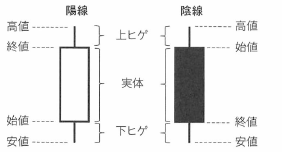
\includegraphics[width=110mm]{fig/candle.png}
  \caption{ローソク足(引用元\cite{pythontrading})}
  \label{fig:candle}
 \end{figure}

 \subsection{日経平均株価}
日経平均株価とは,日本経済新聞社が東京証券取引所プライム市場上場銘柄から選定した225銘柄の株価の平均ことである\cite{nikkei_kabu}.

 \subsection{利益確定}
 利益確定とは,買った株の値段が上がったときに売却し,利益を確定することである.「利食い売り」ともいわれる.ある程度利益を確定して売却することで損失に転換するリスクを可能性を回避できる\cite{rikaku}.
 \subsection{損切り}
損切りとは,損失を抱えている状態で抱えている株を売却して損失を確定させることである.ロスカットやストップロスなどとも呼ばれている.価格が下落し続けている株を保有しておくと損害が大きくなるため,損切りで損失額を抑えることができる\cite{songiri}.
\section{テクニカル指標}
\subsection{MACD(Moving Average Convergence and Divergence)}
% MACD(Moving average Convergence and Divergence)とは短期の移動平均線が中期の移動平均線を下から上に突き抜け,
% かつどちらも横ばいまたは上向きの状態で買いのタイミングとされているゴールデンクロスをもう少し汎用的にしたテクニカル指標のことである.
% MACDでは移動平均が単純移動平均ではなく,直近の価格になるほど比重をおいて計算する平滑移動平均を用いている.
短期と中期の移動平均線がどちらも横ばいか上向きで
あり,短期移動平均線を中期移動平均線が下から上に
突き抜ける買いのタイミングをゴールデンクロスと呼
ぶ.MACD\cite{pythontrading}は,1970年代後半に米国のシグナラート・コーポレーション社の経営者であったジェラルド・アペル氏によって考案された指標であり,
このゴールデンクロスを更に汎用的に
したテクニカル指標である.MACD では移動平均とし
て,単純移動平均ではなく,直近の価格に比重をおく
平滑移動平均を用いる.
MACDは以下の3つの要素で構成されており,各要素の求め方は以下の通りである.
\begin{itemize}
  \item MACD線=X期間の短期移動平均線(EMA) ‐ Y期間の長期移動平均線(EMA)
  \item シグナル線=MACDのZ期間の単純移動平均線(EMA)
  \item ヒストグラム(OSCI)=MACD線 - シグナル線
\end{itemize}
X,Y,Zはパラメータで,本研究ではX=5,Y=20,Z=9を用いる.MACDとシグナルは折れ線グラフで表し,ヒストグラムは棒グラフで表す\cite{pythontrading}.MACDの買いシグナルは,MACD線がシグナル線を下から上に
突き抜ける場合で,売りシグナルは,シグナル線がMACD線を下から上に
突き抜ける場合である.

図\ref{fig:macdex}でMACDの例を示す.この図ではMACDのMACD線,シグナル線,ヒストグラムが示されている.
MACD線がシグナル線が上から下に突き抜けた時に売りシグナルが出ており,売りのタイミングであることがわかる.
同様に,MACD線がシグナル線を下から上に突き抜けたときにシグナルが出ており,買いのタイミングであることがわかる.
ヒストグラムは,売りシグナルのとき正から負になっており,買いシグナルのときは負から正になっていることがわかる.
\begin{figure}[H]
  \centering
  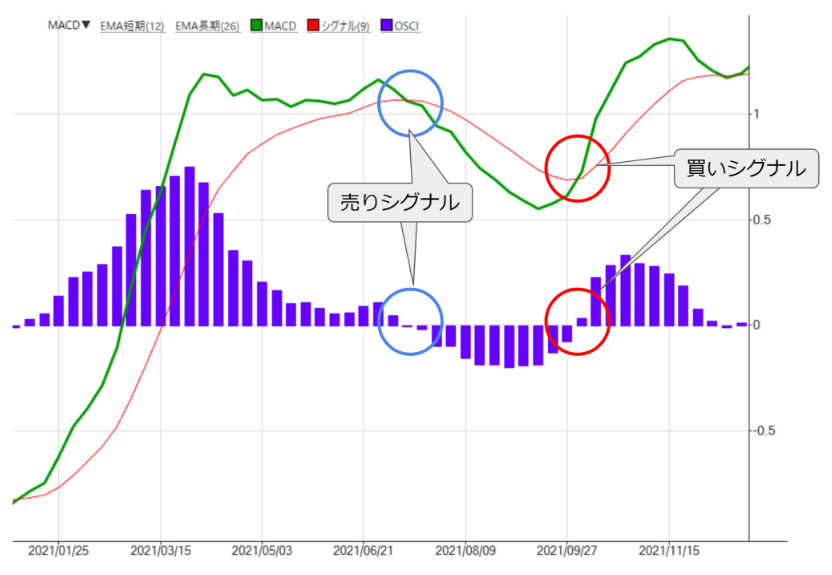
\includegraphics[width=110mm]{fig/macd_exp.png}
  \caption{MACDグラフ(引用元\cite{macdexp})}
  \label{fig:macdex}
 \end{figure}


\subsection{ボリンジャーバンド (BB: Bollinger Band)}
ボリンジャーバンド\cite{pythontrading}とは移動平均線の上下に標準偏差を元に計算された3つのバンドという線を用いるテクニカル指標である.
ボリンジャーバンドの定義式は以下のようになる.
\begin{itemize}
  \item 中央のバンド = $n$日の移動平均線
  \item 上部バンド = 中央のバンド + ($n$日の標準偏差 × X)
  \item 下部バンド = 中央のバンド - ($n$日の標準偏差 × X)
\end{itemize}
nは期間のことであり,本研究では25日を用いている.Xは標準偏差の倍数で1から3までであり,単位はσで扱う.バンドは+1σ (アッパーバンド1), +2σ (アッパーバンド2), +3σ (アッパーバンド3),
-1σ (ロワーバンド1),-2σ (ロワーバンド2), -3σ (ロワーバンド3)の名前で扱う.
株価の変動はバンドの範囲内に収まることが多いと考えられており,ばらつきが多いほど標準偏差は大きくなるため,バンドの幅が広くなる方に値動きが大きくなると判断できる.
株価が収まる確率は以下の通りだとされている\cite{pythontrading}.
\begin{itemize}
  \item ±1σ:68.2%
  \item ±2σ:95.4%
  \item ±3σ:99.7%
\end{itemize}
BBはローソク足とともに表示されることが多く,ローソク足の位置で株価の上がり下がりの余地がどれくらいあるかを判断する.
±3σは±2σとの差が4%しかないため指標としてはあまり重視されない.本論でも±2σをつかって検証する.

図\ref{fig:bbex}はBBの例を示している.移動平均線を基準に±3σ,±2σ,±1σのバンドを示している.BBの買い売りシグナルはいくつかあるが本論では,終値が‐2σを下回ったときに買いシグナルを出すアルゴリズムを提案している.

\begin{figure}[H]
  \centering
  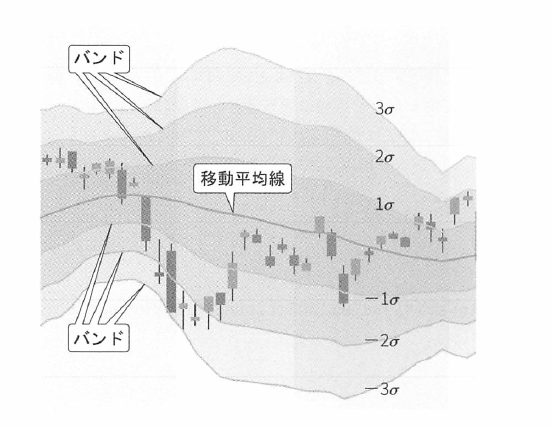
\includegraphics[width=110mm]{fig/bbexp.png}
  \caption{BBグラフ(引用元\cite{pythontrading})}
  \label{fig:bbex}
 \end{figure}
\section{Pythonによるバックテスト環境}

\subsection{Pythonの概要}
% Pythonはオープンソースのインタプリタのオブジェクト指向プログラミング言語で,構文は読みやすく,ライブラリも豊富なため
% 初心者に向いている.コンパイルのステップがないため,編集,テスト,デバッグのサイクルが早い.
% 主な使われている用途としてウェブアプリ,科学的、数値計算,デスクトップGUIで使われている.\cite{pythonapp}
Python\cite{pythontrading,pythonapp,van}は高水準のプログラミング言語であり,直感的で読みやすい構文を持つことが特徴である.1991年にGuido van Rossumによって設計され,その後コミュニティによって発展していった.Pythonは汎用性が高く,ウェブ開発,データ解析,機械学習,人工知能などさまざまな分野で広く利用されている.

Pythonの特徴的な構文として,インデント(行頭の空白文字)を使ったブロック構造があり,これにより可読性が向上し,他のプログラミング言語よりもコードが書きやすい.また,動的型付けを採用しており,変数の型を事前に宣言する必要がないため柔軟性がある.
標準ライブラリが豊富であり,多くの便利なモジュールが組み込まれている.これにより,ファイル操作,ネットワーク通信,データ処理などの様々なタスクを容易に実行することができる.

Pythonはオープンソースで,コミュニティによって広くサポートされており,さらに豊富なドキュメンテーションやオンラインリソースが利用可能であるため,初学者から経験豊富な開発者まで幅広い層に利用されている.
簡潔かつ表現力豊かなコードを書くことができ,初学者にも優しい言語であるため,プログラミングの入門に適している. Pythonは今日では非常に人気があり,多くの大規模なプロジェクトや企業で採用されている.


\subsection{研究で使用するライブラリ}
ここでは研究で用いたライブラリについて説明していく.


\begin{description}
  \item [backtesting\cite{backtesting}]:backtestingは過去の株価データから取引戦略の実行可能性を推測するためのライブラリである.エコシステムライブラリ(Pandas, Numpyなど)の上に構築されているため使いやすく高速に実行可能である.
 
 図\ref{fig:ISMA}のBactestingに含まれている$self.I()$メソッドについて説明する.
 $self.I()$メソッドはインディケータを作成するメソッドで,指定されたインディケータ(ここでは$SMA$)を呼び出し,その結果を取得する.
 $SMA$は単純移動平均を計算する関数である.$self.data$はデータフレームで,
 Date: 日付,Open: 始値,High: 高値,Low: 安値,Close: 終値,Volume: 出来高を格納している.ここでは終値の$self.data["Close"]$を用いている.
 $self.n$は移動平均の期間を指定するパラメータである.
 つまりこのメソッドの引数には,$n$期間の終値の単純移動平均がか与えられている.
  
   図\ref{fig:cros}のcrossoverメソッドについて説明する.このメソッドは交差するかどうかを判定する関数である.この場合,
   \( self.b\_lower \)が,$self.data["Close"]$より下から上に交差した場合,Trueを返す関数となっている.
   

   図\ref{fig:strat}について説明する.class bbはBactestingのStrategyクラスを継承して,独自の売買戦略を定義している.
   パラメータや変数は提案するアルゴリズムによって定義する.ここでは\( n \),\( n1 \), \( n2 \), \( n3 \), \( nb \), \( upper\_sigma \), \( lower\_sigma \), \( slinit \), \( tpinit \)を定義している.
   
   def init(self)は,初期化メソッドで,図\ref{fig:ISMA}と同じように
   MACD,BBを取得し,\(self.macd\),\(self.macdsignal\),\(self.b\_upper\),\(self.b\_lower\)に格納している.また,損切りのパラメータの\( slinit \)と 利確のパラメータの\( tpinit \)を初期化している.

   def next(self)メソッドは,時間単位で呼び出され,条件で売買を行う.ここでは図\ref{fig:cros}で説明したcrossoverメソッドを用いて真偽値を出している.真である場合,self.buyメソッドを呼び出して買い注文をしている.
   \( slinit \)と \( tpinit \)をもちいて売却の条件も設定している.
   \begin{figure}[H]
    \centering
    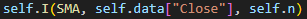
\includegraphics[width=110mm]{fig/I_SMA.png}
    \caption{インディケータメソッド,SMA,self.data}
    \label{fig:ISMA}
   \end{figure}

   \begin{figure}[H]
       \centering
       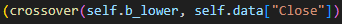
\includegraphics[width=110mm]{fig/crossover.png}
       \caption{クロスオーバーメソッド}
       \label{fig:cros}
      \end{figure}
      \begin{figure}[H]
        \centering
        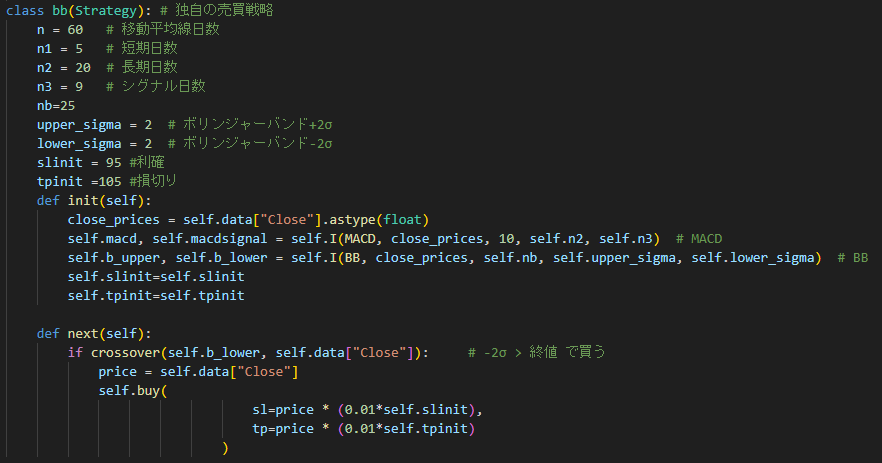
\includegraphics[width=150mm]{fig/strategy.png}
        \caption{売買戦略}
        \label{fig:strat}
       \end{figure}
    

   図\ref{fig:databt}について説明する.\(s\_code\)は銘柄コードを格納しており,dfは独自の\(get\_stock\_data\_from\_file()\)から取得した株価データを格納している.$data$は取得した株価データの2013年1月1日から
   2022年12月31日までの株価データを保持している.
   
   $bt$はBactestingのBacktestクラスを用いてバックテストを初期化する.ここで使用しているのは先ほど説明した$data$,図\ref{fig:strat}で説明した戦略と取引をクローズ時に行うかどうかの設定
   の\(trade\_on\_close\)で,Trueの場合はクローズ時に取引が行われる.

   $result$は$optimize$メソッドで$bt$を最適化している.ここで最適化するパラメータは\(slinit\)と\(tpinit\)で,\(slinit\)は90から100まで1単位,\(tpinit\)は101から110まで1単位で試行する.
   このとき\( Return[\%]\),つまり利益率を最大化するように設定する.
   \begin{figure}[H]
    \centering
    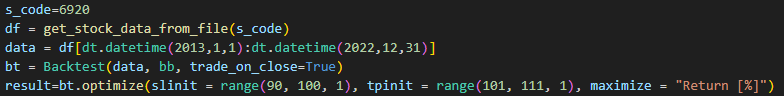
\includegraphics[width=150mm]{fig/data_bt_result.png}
    \caption{バックテスト}
    \label{fig:databt}
   \end{figure}
   図\ref{fig:resbt}に付いて説明する.この図はバックテストを行って最適化実行時の結果である.pandas.DataFrame型のオブジェクトである.ここでは本研究で使用する実行結果のデータは,以下の通りである.
   \begin{description}
    \item[Return[\%]]:10年間の利益率
    \item [\# Trade]:10年間の取引数
    \item [Win Rate[\%]]:10年間の勝率
   \end{description}
   \item [datetime]:datetimeは日時に関するデータを操作するためのクラスを提供している\cite{datetime}.図\ref{fig:datetest}と図\ref{fig:dateres}に簡単な使用例と実行結果を示す.$datetime.now()$メソッドを使って,現在の日付と時刻と取得し,$current\_datetime$に格納している.そのあと$print()$関数で結果を出力する.
  実行結果は図\ref{fig:dateres}のようになる.





  
   
  \item [pandas]:pandasはデータを簡単かつ直感的に扱えるように設計されたデータ構造を提供している\cite{pandas}.
  図\ref{fig:pdtest}と図\ref{fig:pdres}に簡単な使用例と実行結果を示す.辞書型(dictionary)としてデータを定義する.キーとして'Name','Age','City'があり,それぞれのキーに対応する値がリストとして格納されている.
  辞書型のデータを用いてPandasのDataFrameを作成する.DataFrameは表形式のデータ構造で,ここでは'Name','Age','City'の列を持つ3つの行が作成される.そのあと$print()$関数で結果を出力する.実行結果は図\ref{fig:pdres}のようになる.

  \item [numpy]:numPy は,Python を使用した科学技術コンピューティング用のライブラリである\cite{numpy}.図\ref{fig:nptest}と図\ref{fig:npres}に簡単な使用例と実行結果を示す.
  NumPyのarray関数を用いて与えられたリスト$[[1, 2, 3], [4, 5, 6]]$より2次元のNumPy配列を作成する.そのあと$print()$関数で結果を出力する.実行結果は図\ref{fig:npres}のようになる.
  \begin{figure}[H]
    \centering
    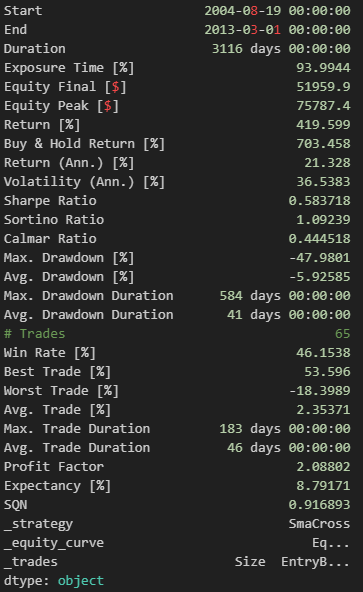
\includegraphics[width=100mm]{fig/bt_res.png}
    \caption{バックテスト実行時の結果}
    \label{fig:resbt}
   \end{figure}

   \begin{figure}[H]
    \centering
    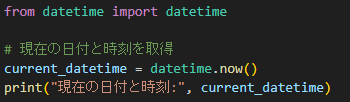
\includegraphics[width=110mm]{fig/datetime_test.png}
    \caption{datetimeの使用例}
    \label{fig:datetest}
   \end{figure}
  
   \begin{figure}[H]
    \centering
    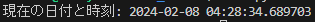
\includegraphics[width=110mm]{fig/datetime_res.png}
    \caption{図\ref{fig:datetest}実行時の結果}
    \label{fig:dateres}
   \end{figure}
  %%%%%%%%%%%%%%%%%%%%%%%%%%%%%%%%%%%%%%%%%%%%%%%%%%%
  
  \begin{figure}[H]
    \centering
    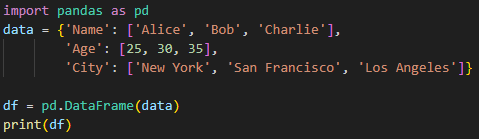
\includegraphics[width=110mm]{fig/pandas_test.png}
    \caption{pandasの使用例}
    \label{fig:pdtest}
   \end{figure}
  
   \begin{figure}[H]
    \centering
    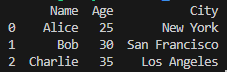
\includegraphics[width=80mm]{fig/pandas_res.png}
    \caption{図\ref{fig:pdtest}実行時の結果}
    \label{fig:pdres}
   \end{figure}

   \begin{figure}[H]
    \centering
    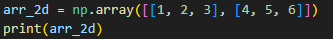
\includegraphics[width=110mm]{fig/np_test.png}
    \caption{numpyの使用例}
    \label{fig:nptest}
   \end{figure}

   \begin{figure}[H]
    \centering
    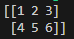
\includegraphics[width=30mm]{fig/np_res.png}
    \caption{図\ref{fig:nptest}実行時の結果}
    \label{fig:npres}
   \end{figure}
  \item [talib]:talibは金融取引で使われている指標のライブラリを提供している\cite{talib}.図\ref{fig:talibtest}と図\ref{fig:talibres}に簡単な使用例と実行結果を示す.
NumPyのrandom関数を用いて,0から1までのランダムな数値を100個生成し,それぞれに100を掛けて仮想の株価データを制作する.Ta-LibのSMA関数を用いて,与えられた株価データに対して20期間の単純移動平均を計算する.そのあと$print()$関数で結果を出力する.
実行結果は図\ref{fig:talibtest}のようになる.


  \item [matplotlib]:matplotlibはアニメーションやグラフを作成するために使われるライブラリである\cite{matplotlib}.図\ref{fig:plttest}と図\ref{fig:pltres}に簡単な使用例と実行結果を示す.
  NumPyのlinspace関数を用いて,0から10までの範囲を100点で均等に区切ったデータを生成する.NumPyのsin関数を用いて,各$x$に対する$sin(x)$の値を計算する.$plt.plot()$メソッドで折れ線グラフをプロットする.
  $plt.title()$メソッドでグラフにタイトルを追加する.$plt.xlabe()$メソッドと$plt.ylabel()$メソッドで x軸とy軸にラベルを追加する.$plt.legend()$メソッドでグラフにを表示する.$plt.show()$メソッドで,
  作成したグラフを表示する.実行結果は図\ref{fig:pltres}のようになる.



 
   %%%%%%%%%%%%%%%%%%%%%%%%%%%%%%%%%%%%%%%%%%%%%%%
 
   %%%%%%%%%%%%%%%%%%%%%%%%%%%%%%%%%%%%%%%%%%%%%

%%%%%%%%%%%%%%%%%%%%%%%%%%%%%%%%%%%%%%%%%%%%%%%%%%
  \begin{figure}[H]
    \centering
    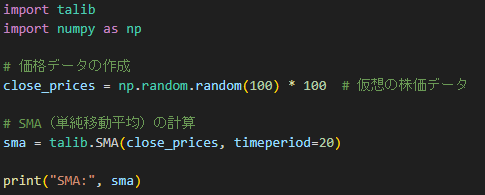
\includegraphics[width=110mm]{fig/talib_test.png}
    \caption{talibの使用例}
    \label{fig:talibtest}
   \end{figure}

   \begin{figure}[H]
    \centering
    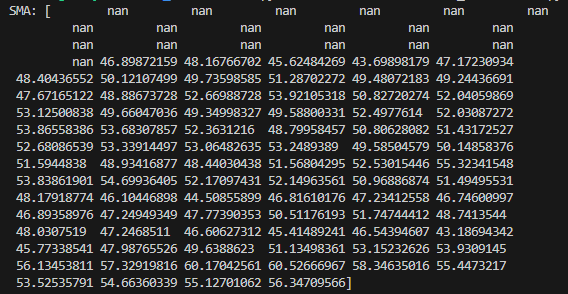
\includegraphics[width=110mm]{fig/talib_res.png}
    \caption{図\ref{fig:talibtest}実行時の結果}
    \label{fig:talibres}
   \end{figure}
   %%%%%%%%%%%%%%%%%%%%%%%%%%%%%%%%%%%%%%%%%%%%%%%%%%
  \begin{figure}[H]
    \centering
    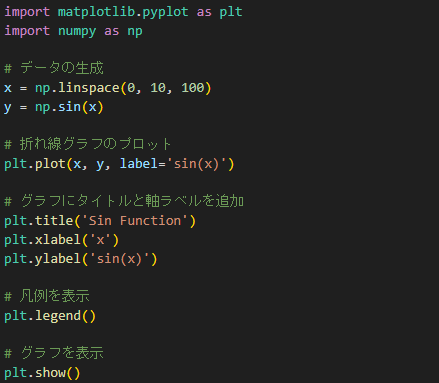
\includegraphics[width=110mm]{fig/plt_test.png}
    \caption{matplotlibの使用例}
    \label{fig:plttest}
   \end{figure}

   \begin{figure}[H]
    \centering
    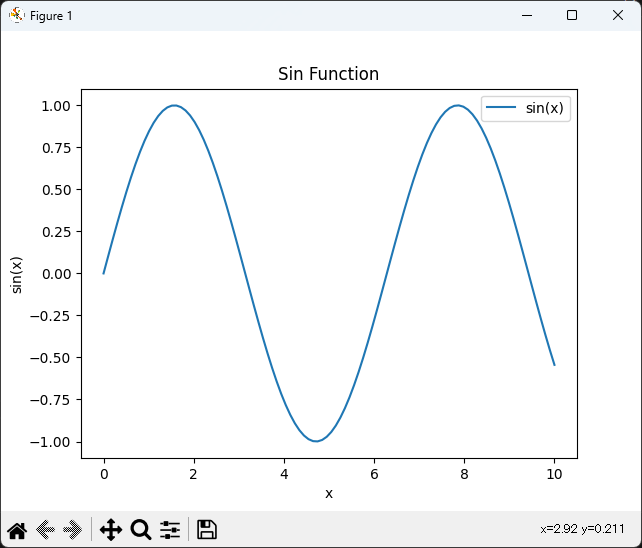
\includegraphics[width=110mm]{fig/plt_res.png}
    \caption{図\ref{fig:plttest}実行時の結果}
    \label{fig:pltres}
   \end{figure}
   %%%%%%%%%%%%%%%%%%%%%%%%%%%%%%%%%%%%%%%%%%%%%%%%%%
\end{description}


\newpage
\chapter{トレーディングアルゴリズム}
本章では,実際に使うトレーディングアルゴリズムを順に説明する.
\section{MACD}
ここではMACDを主に使うトレーディングアルゴリズムの説明をする.利確時の変数$tp$および損切り時の変数$sl$はアルゴリズム実行時,変更可能なパラメータである.

\subsection{MACDのみ}
MACDのみを使う場合のトレーディングアルゴリズムの説明をする.ここでは(B1)とする.
\begin{description}
\item[\textbf{Step~1~:}]MACDがシグナルを下から上へ突き抜けたときに翌日の始値で株を購入する.

\item[\textbf{Step~2~:}]以下の(2-1)~(2-2)のどちらかの条件が満たされれば売却する.
 \begin{description}
  \item[\textbf{(2-1):}]株の始値が購入した株価より$tp$%以上になった時点で売る.
  \item[\textbf{(2-2):}]株の始値が購入した株価より$sl$%以下になった時点で売る. 
 \end{description}
\item[\textbf{Step~3~:}]用意した株価データの最終日が来るまでStep 1からStep 3まで繰り返す.
\end{description}


図\ref{fig:macdonly}にMACDによる買いシグナルの例を示す.図\ref{fig:macdonly}の黒丸がMACDの買いシグナルで,その後$tp$%以上で売っている.
%%%%%%%%%%%%%%%%%

\subsection{MACDと60日移動平均線}
MACDと60日移動平均線を使う場合のトレーディングアルゴリズムを説明する.
長期の移動平均線の傾きが正の場合,株価も上昇する傾向にあるため,
MACDと組み合わせることで取引の勝率が上がると考えられ,それにより最終利益が増加すると想定している.
このアルゴリズムでは,60日平均線を長期線とする.ここでは(B2)とする.

\begin{figure}[t]
  \centering
  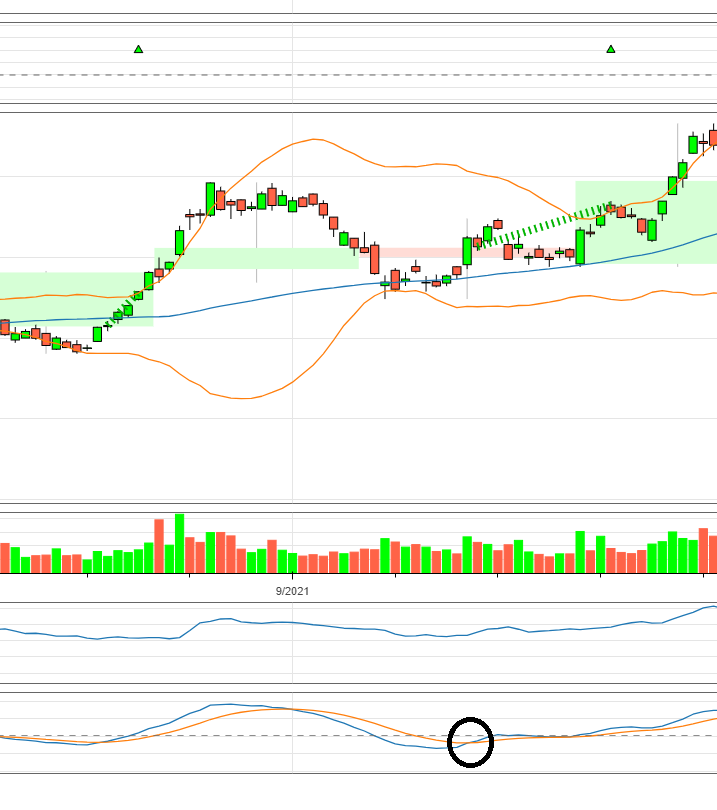
\includegraphics[width=110mm]{fig/macdonly.png}
  \caption{(B1)アルゴリズムの買いシグナル}
  \label{fig:macdonly}
 \end{figure}
\begin{description}
  \item[\textbf{Step~1~:}]以下の(1-1)~(1-2)のすべての条件が満たされれば翌日購入するする.
  \begin{description}
    \item[\textbf{(1-1):}]MACDがシグナルを下から上へ突き抜けたとき.
    \item[\textbf{(1-2):}]長期線の傾きが0以上のとき.
   \end{description}  
  
  \item[\textbf{Step~2~:}]以下の(2-1)~(2-2)のどちらかの条件が満たされれば売却する.
   \begin{description}
    \item[\textbf{(2-1):}]株の始値が購入した株価より$tp$%以上になった時点で売る.
    \item[\textbf{(2-2):}]株の始値が購入した株価より$sl$%以下になった時点で売る. 
   \end{description}
  \item[\textbf{Step~3~:}]用意した株価データの最終日が来るまでStep 1からStep 3まで繰り返す.
  \end{description}
  
   図\ref{fig:macdfma}にMACDと長期線よる買いシグナルの例を示す.図\ref{fig:macdfma}の黒丸がMACDの買いシグナルで,その時の長期線の傾きも0以上なので購入している.その後$tp$%以上で売っている.
   \begin{figure}[t]
    \centering
    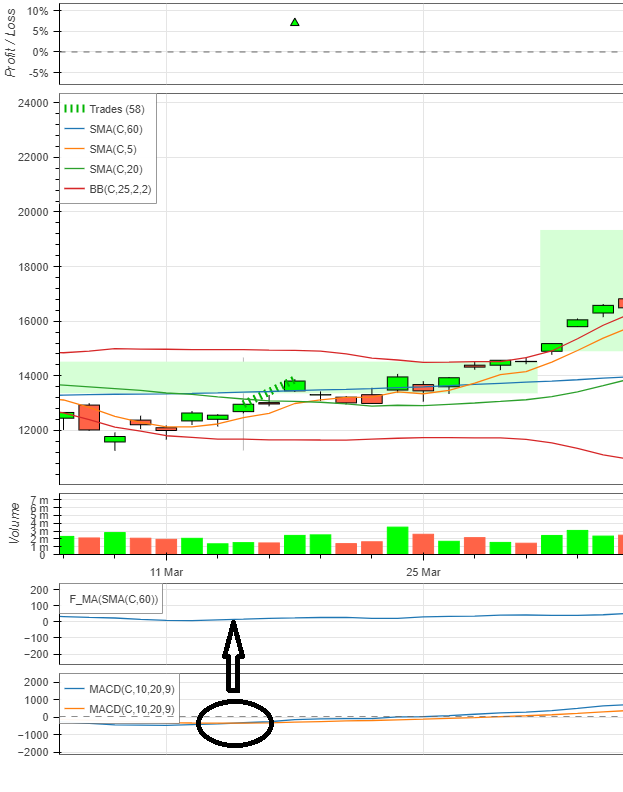
\includegraphics[width=110mm]{fig/macd_fma.png}
    \caption{(B2)アルゴリズムの買いシグナル}
    \label{fig:macdfma}
   \end{figure}

   %%%%%%%%%%%%%%%%%%

\subsection{MACDと日経株価平均}
MACDと日経平均株価を使う場合のトレーディングアルゴリズムを説明する.
日経株価平均は日本の主要な225銘柄を対象としており,日経株価平均が上昇しているということは市場全体が安定していると考えられ,
投資家の信頼があることを示唆している.つまり東証上位100社にもこの安定性が影響を及ぼすと考えられ,
それにより最終利益が増加すると想定している.
ここでは(B3)とする.
\begin{description}
  \item[\textbf{Step~1~:}]以下の(1-1)~(1-2)のすべての条件が満たされれば翌日購入するする.
  \begin{description}
    \item[\textbf{(1-1):}]注目する日のMACDがシグナルを下から上へ突き抜けたとき.
    \item[\textbf{(1-2):}]注目する日の日経平均株価の長期線の傾きが0以上のとき.
   \end{description}  
  
  
  \item[\textbf{Step~2~:}]以下の(2-1)~(2-2)のどちらかの条件が満たされれば売却する.
   \begin{description}
    \item[\textbf{(2-1):}]株の始値が購入した株価より$tp$%以上になった時点で売る.
    \item[\textbf{(2-2):}]株の始値が購入した株価より$sl$%以下になった時点で売る. 
   \end{description}
  \item[\textbf{Step~3~:}]用意した株価データの最終日が来るまでStep 1からStep 3まで繰り返す.
  \end{description}
  
   図\ref{fig:macdnk}にMACDと日経株価平均による買いシグナルの例を示す.図\ref{fig:macdnk}の黒丸がMACDの買いシグナルで,その時の日経株価平均の傾きも0以上なので購入している.その後$tp$%以上で売っている.


   %%%%%%%%%%%%%%%%%%

\subsection{MACDと日経株価平均と長期線}
MACDと日経平均株価と取引している株価データの長期線を使う場合のトレーディングアルゴリズムを説明する.
日経平均株価と取引している株価データの長期線を組み合わせることで,より勝率が上がると考えられ,
(B2),(B3)よりも最終利益が増加すると想定している.
ここでは二通りの方法を説明する.最初に説明するアルゴリズムを(B4),その後に説明するアルゴリズムを(B5)とする.


\begin{description}
    \item [\textbf{(B4):}]
    \item[\textbf{Step~1~:}]以下の(1-1)~(1-3)のすべての条件が満たされれば翌日購入するする.
    \begin{description}
      \item[\textbf{(1-1):}]注目する日のMACDがシグナルを下から上へ突き抜けたとき.
      \item[\textbf{(1-2):}]注目する日の日経平均株価の長期線の傾きが0以上のとき.
      \item[\textbf{(1-3):}]取引している株価データの長期線の傾きが0以上のとき. 
     \end{description}  
    
    
    \item[\textbf{Step~2~:}]以下の(2-1)~(2-2)のどちらかの条件が満たされれば売却する.
     \begin{description}
      \item[\textbf{(2-1):}]株の始値が購入した株価より$tp$%以上になった時点で売る.
      \item[\textbf{(2-2):}]株の始値が購入した株価より$sl$%以下になった時点で売る. 
     \end{description}
    \item[\textbf{Step~3~:}]用意した株価データの最終日が来るまでStep 1からStep 3まで繰り返す.

  \end{description}
    
     図\ref{fig:macdfmank}にMACD,長期線,日経株価平均による買いシグナルの例を示す.図\ref{fig:macdfmank}の黒丸がMACDの買いシグナルで,その上に表示されているその時の長期線の傾きと更に上の日経株価平均の傾きも0以上なので購入している.その後$tp$%以上で売っている.
  \begin{description}
    \begin{figure}[t]
      \centering
      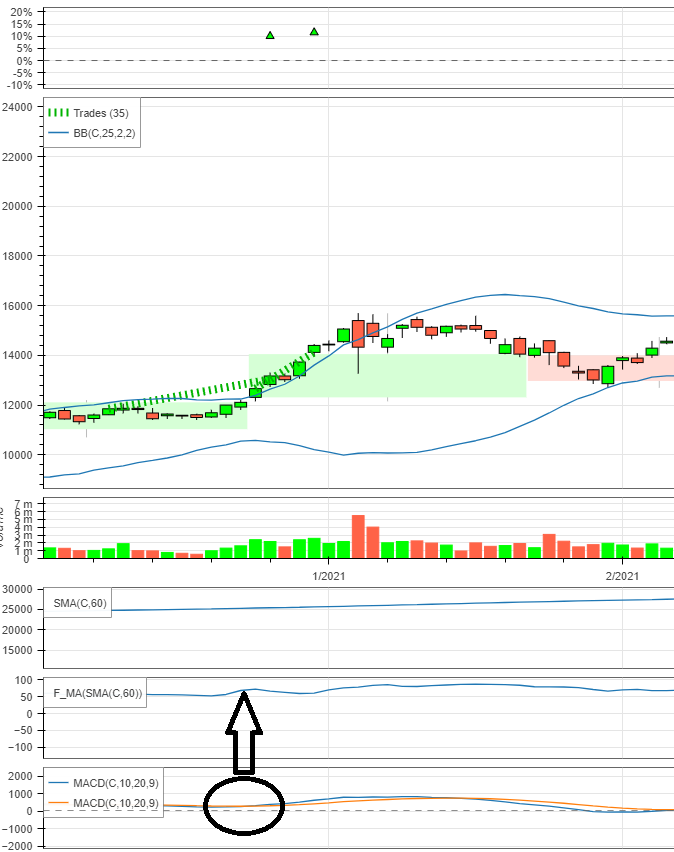
\includegraphics[width=110mm]{fig/macd_nk_paint.png}
      \caption{(B3)アルゴリズムの買いシグナル}
      \label{fig:macdnk}
     \end{figure}
    
    \item [\textbf{(B5):}]
    \item[\textbf{Step~1~:}]以下の(1-1)の条件と(1-2),(1-3)のどちらかの条件が満たされれば翌日購入するする.
    \begin{description}
      \item[\textbf{(1-1):}]注目する日のMACDがシグナルを下から上へ突き抜けたとき.
      \item[\textbf{(1-2):}]注目する日の日経平均株価の長期線の傾きが0以上のとき.
      \item[\textbf{(1-3):}]取引している株価データの長期線の傾きが0以上のとき. 

     \end{description}  
    
    
    \item[\textbf{Step~2~:}]以下の(2-1)~(2-2)のどちらかの条件が満たされれば売却する.
     \begin{description}
      \item[\textbf{(2-1):}]株の始値が購入した株価より$tp$%以上になった時点で売る.
      \item[\textbf{(2-2):}]株の始値が購入した株価より$sl$%以下になった時点で売る. 
     \end{description}
     \begin{figure}[H]
      \centering
      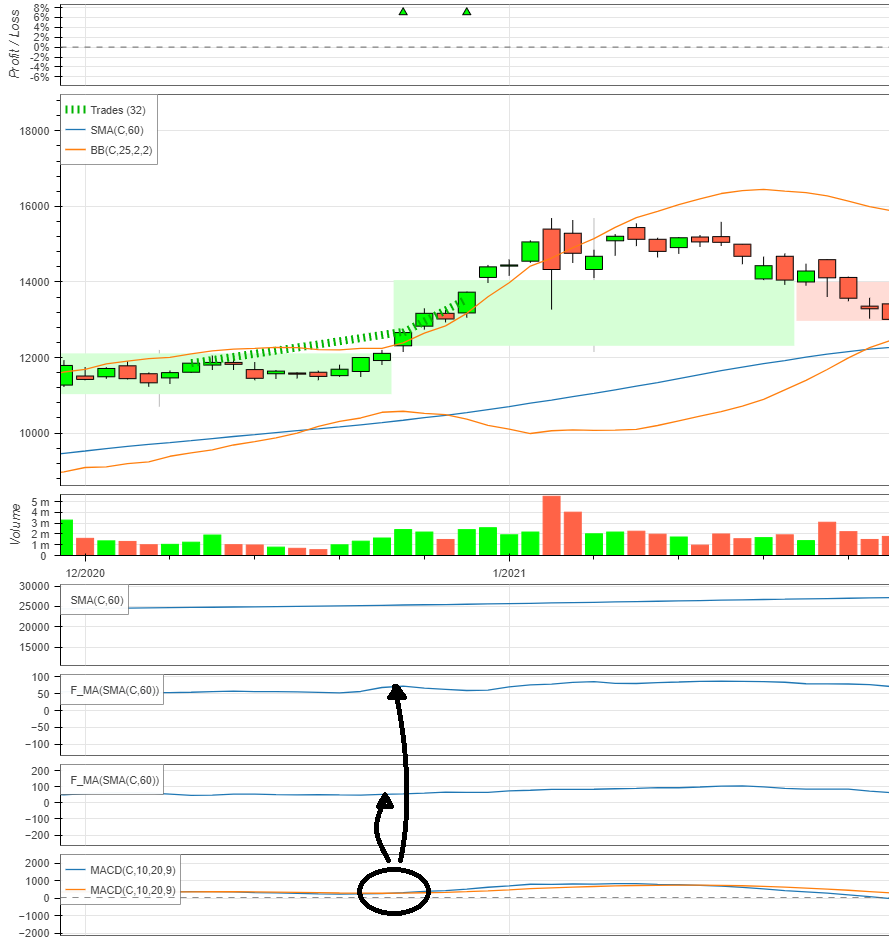
\includegraphics[width=110mm]{fig/macd_and_nk_and_fma_paint.png}
      \caption{(B4)アルゴリズムの買いシグナル}
      \label{fig:macdfmank}
     \end{figure}
    \item[\textbf{Step~3~:}]用意した株価データの最終日が来るまでStep 1からStep 3まで繰り返す.
\end{description}

  
 図\ref{fig:macdfma0nk},図\ref{fig:macdfmank0}に(B5)アルゴリズムの買いシグナルの例を示す.図\ref{fig:macdfma0nk}の黒丸がMACDの買いシグナルで,その時の赤丸の長期線の傾きは0以下だが青丸の日経株価平均の傾きが0以上なので購入している.その後$tp$%以上で売っている.
 また図\ref{fig:macdfmank0}の黒丸がMACDの買いシグナルで,その時の青丸の日経株価平均の傾きは0以下だが赤丸の長期線の傾きが0以上なので購入している.その後$tp$%以上で売っている.
%%%%%%%%%%%%%%%%%%
\section{BB}
ここではBBを主に使うトレーディングアルゴリズムの説明をする.利確時の変数$tp$および損切り時の変数$sl$はアルゴリズム実行時,変更可能なパラメータである.
\begin{figure}[t]
  \centering
  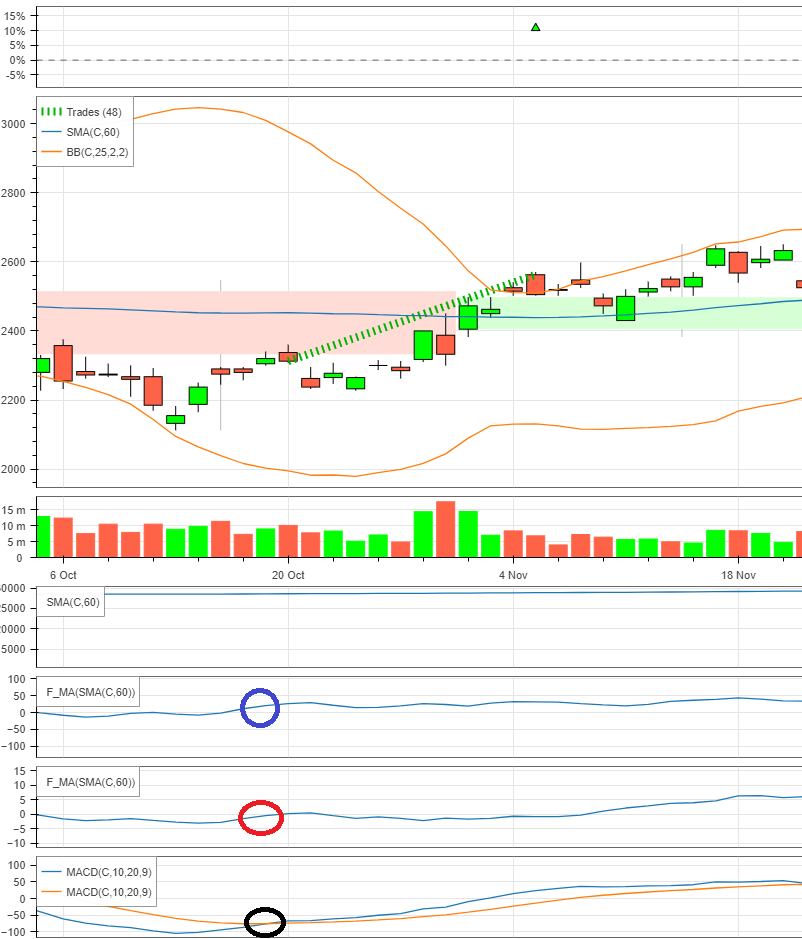
\includegraphics[width=110mm]{fig/macd_and_nk_or_fma0_6857_paint.png}
  \caption{(B5)アルゴリズムの(1-1)と(1-2)の買いシグナル}
  \label{fig:macdfma0nk}
 \end{figure}

 \begin{figure}[t]
  \centering
  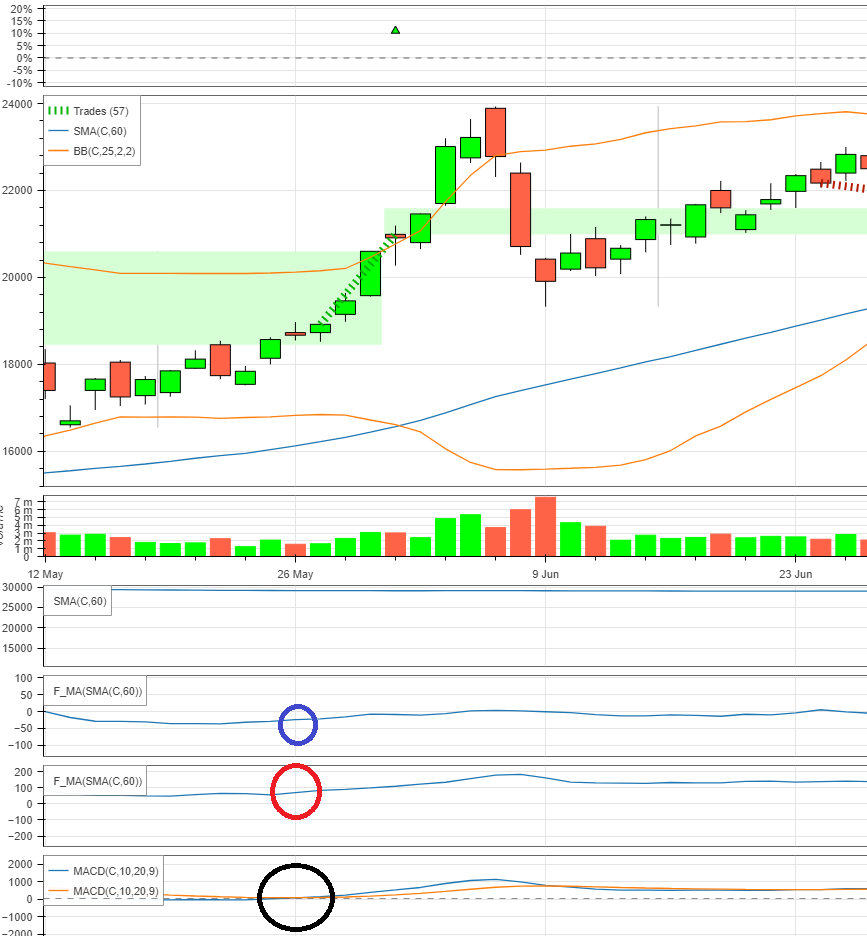
\includegraphics[width=110mm]{fig/macd_and_nk0_or_fma_paint.png}
  \caption{(B5)アルゴリズムの(1-1)と(1-3)の買いシグナル}
  \label{fig:macdfmank0}
 \end{figure}
\subsection{BBのみ}
BBのみを使う場合のトレーディングアルゴリズムの説明をする.ここでは(B6)とする.
\begin{description}
\item[\textbf{Step~1~:}]注目する日のローソクの終値が-2σのBBを上から下へ突き抜けたときに終値で株を購入する.

\item[\textbf{Step~2~:}]以下の(2-1)~(2-2)のどちらかの条件が満たされれば売却する.
 \begin{description}
  \item[\textbf{(2-1):}]株の始値が購入した株価より$tp$%以上になった時点で売る.
  \item[\textbf{(2-2):}]株の始値が購入した株価より$sl$%以下になった時点で売る. 
 \end{description}
\item[\textbf{Step~3~:}]用意した株価データの最終日が来るまでStep 1からStep 3まで繰り返す.
\end{description}

  
 図\ref{fig:bbonly}にBBによる買いシグナルの例を示す.図\ref{fig:bbonly}の黒丸がBBの買いシグナルで,その後$tp$%以上で売っている.
%%%%%%%%%%%%%%%%%%
\subsection{BBと60移動平均線}
BBと移動平均線を使う場合のトレーディングアルゴリズムの説明をする.60移動平均線を組み合わせる理由として(B2)と同じように,
取引の勝率が上がると考えられ,それにより最終利益が増加すると想定している.
ここでは(B7)とする.
\begin{description}
  \item[\textbf{Step~1~:}]以下の(1-1)~(1-2)のすべての条件が満たされれば終値で購入する.
  \begin{description}
    \item[\textbf{(1-1):}]注目する日のローソクの終値が-2σのBBを上から下へ突き抜けたときに終値で株を購入する.
    \item[\textbf{(1-2):}]長期線の傾きが0以上のとき.
   \end{description}  
   \begin{figure}[t]
    \centering
     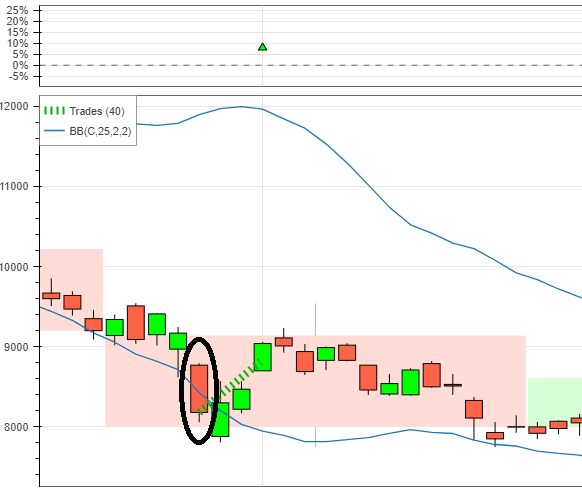
\includegraphics[width=110mm]{fig/bbonly_paint.png}
     \caption{(B6)アルゴリズムの買いシグナル}
     \label{fig:bbonly}
    \end{figure}
  \item[\textbf{Step~2~:}]以下の(2-1)~(2-2)のどちらかの条件が満たされれば売却する.
   \begin{description}
    \item[\textbf{(2-1):}]株の始値が購入した株価より$tp$%以上になった時点で売る.
    \item[\textbf{(2-2):}]株の始値が購入した株価より$sl$%以下になった時点で売る. 
   \end{description}
  \item[\textbf{Step~3~:}]用意した株価データの最終日が来るまでStep 1からStep 3まで繰り返す.
  \end{description}
  
   図\ref{fig:bbfma}にBBと長期線による買いシグナルの例を示す.図\ref{fig:bbfma}の黒丸がBBの買いシグナルで,その時の赤丸の長期線の傾きは0以上なので購入している.その後$tp$%以上で売っている.
%%%%%%%%%%%%%%%%%%
\subsection{BBと日経平均株価}
BBと日経平均株価を使う場合のトレーディングアルゴリズムの説明をする.日経平均株価を組み合わせる理由として(B3)と同じように,
取引の勝率が上がると考えられ,それにより最終利益が増加すると想定している.ここでは(B8)とする.
\begin{description}
  \item[\textbf{Step~1~:}]以下の(1-1)~(1-2)のすべての条件が満たされれば翌日購入するする.
  \begin{description}
    \item[\textbf{(1-1):}]注目する日のローソクの終値が-2σのBBを上から下へ突き抜けたときに終値で株を購入する.
    \begin{figure}[t]
      \centering
      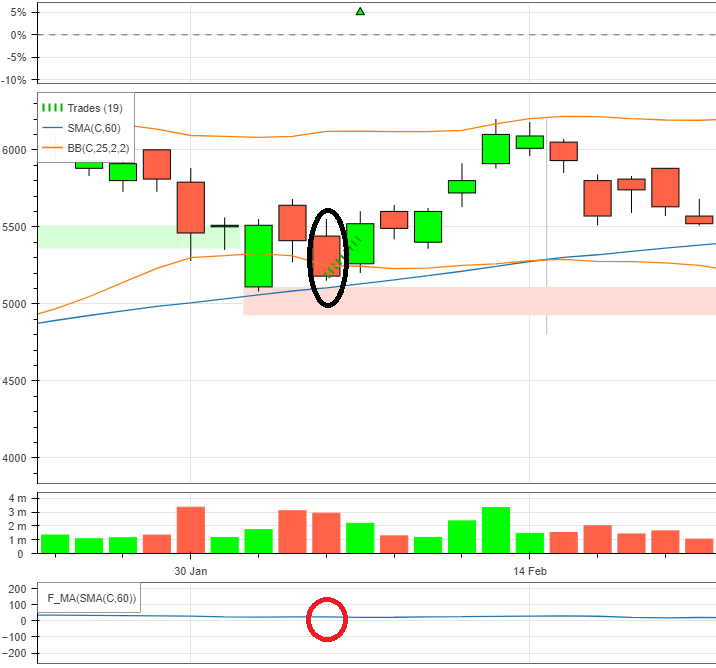
\includegraphics[width=110mm]{fig/bb_fma_paint.png}
      \caption{(B7)アルゴリズムの買いシグナル}
      \label{fig:bbfma}
     \end{figure}
    \item[\textbf{(1-2):}]注目する日の日経平均株価の長期線の傾きが0以上のとき.
   \end{description}  
  
  \item[\textbf{Step~2~:}]以下の(2-1)~(2-2)のどちらかの条件が満たされれば売却する.
   \begin{description}
    \item[\textbf{(2-1):}]株の始値が購入した株価より$tp$%以上になった時点で売る.
    \item[\textbf{(2-2):}]株の始値が購入した株価より$sl$%以下になった時点で売る. 
   \end{description}
  \item[\textbf{Step~3~:}]用意した株価データの最終日が来るまでStep 1からStep 3まで繰り返す.
  \end{description}
  
   図\ref{fig:bbnk}にBBと日経株価平均による買いシグナルの例を示す.図\ref{fig:bbnk}の黒丸がBBの買いシグナルで,その時の赤丸の日経株価平均の傾きは0以上なので購入している.その後$tp$%以上で売っている.
%%%%%%%%%%%%%%%%%%

\subsection{BBと日経株価平均と長期線}
BBと日経平均株価と取引している株価データの長期線を使う場合のトレーディングアルゴリズムを説明する. (B4),(B5)同じように,取引の勝率が上がると考
えられ,それにより最終利益が増加すると想定している.
ここでは二通りの方法を説明する.最初に説明するアルゴリズムを(B9),その後に説明するアルゴリズムを(B10)とする.
\begin{figure}[t]
  \centering
  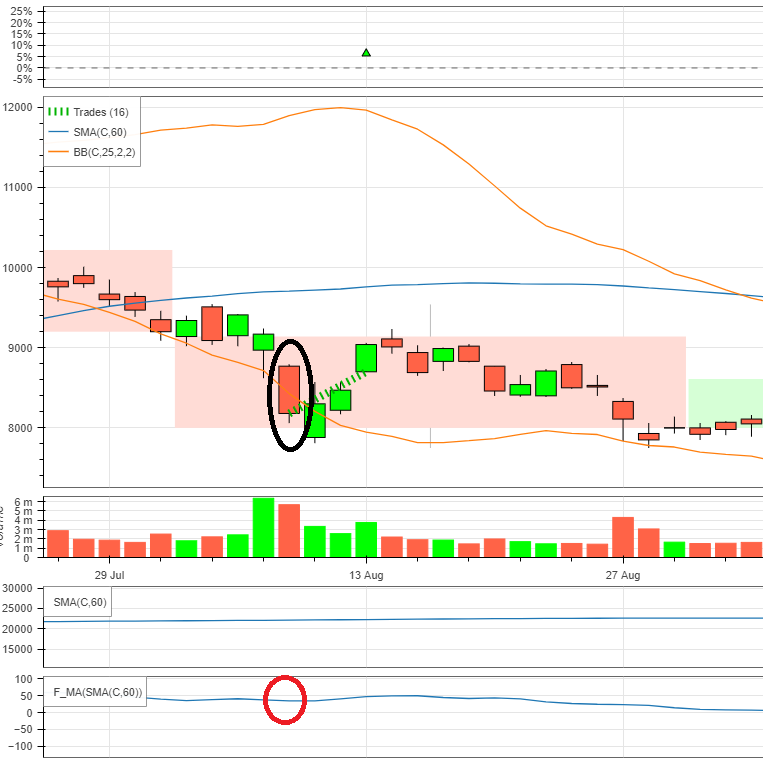
\includegraphics[width=110mm]{fig/bb_nk_paint.png}
  \caption{(B8)アルゴリズムの買いシグナル}
  \label{fig:bbnk}
 \end{figure}
\begin{description}
  \item[\textbf{(B9):}]
    \item[\textbf{Step~1~:}]以下の(1-1)~(1-3)のすべての条件が満たされれば翌日購入するする.
    \begin{description}
      \item[\textbf{(1-1):}]注目する日のローソクの終値が-2σのBBを上から下へ突き抜けたときに終値で株を購入する.
      \item[\textbf{(1-2):}]注目する日の日経平均株価の長期線の傾きが0以上のとき.
      \item[\textbf{(1-3):}]取引している株価データの長期線の傾きが0以上のとき. 
     
    \item[\textbf{Step~2~:}]以下の(2-1)~(2-2)のどちらかの条件が満たされれば売却する.
     \begin{description}
      \item[\textbf{(2-1):}]株の始値が購入した株価より$tp$%以上になった時点で売る.
      \item[\textbf{(2-2):}]株の始値が購入した株価より$sl$%以下になった時点で売る. 
     \end{description}
    \item[\textbf{Step~3~:}]用意した株価データの最終日が来るまでStep 1からStep 3まで繰り返す.
    \end{description}
  \end{description}  
 
   
  図\ref{fig:bbnkfma}にBB,長期線,日経株価平均による買いシグナルの例を示す.図\ref{fig:bbnkfma}の黒丸がBBの買いシグナルで,その時の長期線の傾きと日経株価平均の傾きも0以上なので購入している.その後$tp$%以上で売っている.

  \begin{description}
    \item[\textbf{(B10):}]
    \item[\textbf{Step~1~:}]以下の(1-1)の条件と(1-2),(1-3)のどちらかの条件が満たされれば終値で購入する.
    \begin{description}
      \item[\textbf{c:}]注目する日のローソクの終値が-2σのBBを上から下へ突き抜けたときに終値で株を購入する.
      \item[\textbf{(1-2):}]注目する日の日経平均株価の長期線の傾きが0以上のとき.
      \item[\textbf{(1-3):}]取引している株価データの長期線の傾きが0以上のとき. 

     \end{description}  
    
    
    \item[\textbf{Step~2~:}]以下の(2-1)~(2-2)のどちらかの条件が満たされれば売却する.
     \begin{description}
      \item[\textbf{(2-1):}]株の始値が購入した株価より$tp$%以上になった時点で売る.
      \item[\textbf{(2-2):}]株の始値が購入した株価より$sl$%以下になった時点で売る. 
     \end{description}
    \item[\textbf{Step~3~:}]用意した株価データの最終日が来るまでStep 1からStep 3まで繰り返す.
    \end{description}
    
     図\ref{fig:bbnkfma0},及び,図\ref{fig:bbnk0fma}に,(B10)アルゴリズムによる買いシグナルの例を示す.図\ref{fig:bbnkfma0}の黒丸がBBの買いシグナルで,その時の赤丸の長期線の傾きは0以下だが青丸の日経株価平均の傾きが0以上なので購入している.その後$tp$%以上で売っている.
 また図\ref{fig:bbnk0fma}の黒丸がBBの買いシグナルで,その時の青丸の日経株価平均の傾きは0以下だが赤丸の長期線の傾きが0以上なので購入している.その後$tp$%以上で売っている.
%%%%%%%%%%%%%%%%%%%%%%%%%%%%%%%%%%%%%%%%%%%%%%%%%%%%%%%%%%%%%%%
\section{MACDとBB}
ここではMACDとBBを主に使うトレーディングアルゴリズムの説明をする.利確時の変数$tp$および損切り時の変数$sl$はアルゴリズム実行時,変更可能なパラメータである.
\subsection{MACDとBB}
MACDとBBを使う場合のトレーディングアルゴリズムを説明する.2つを組み合わせることでより良い効果が得られるのではないかと想定している.ここでは(B11)とする.
\begin{figure}[H]
  \centering
    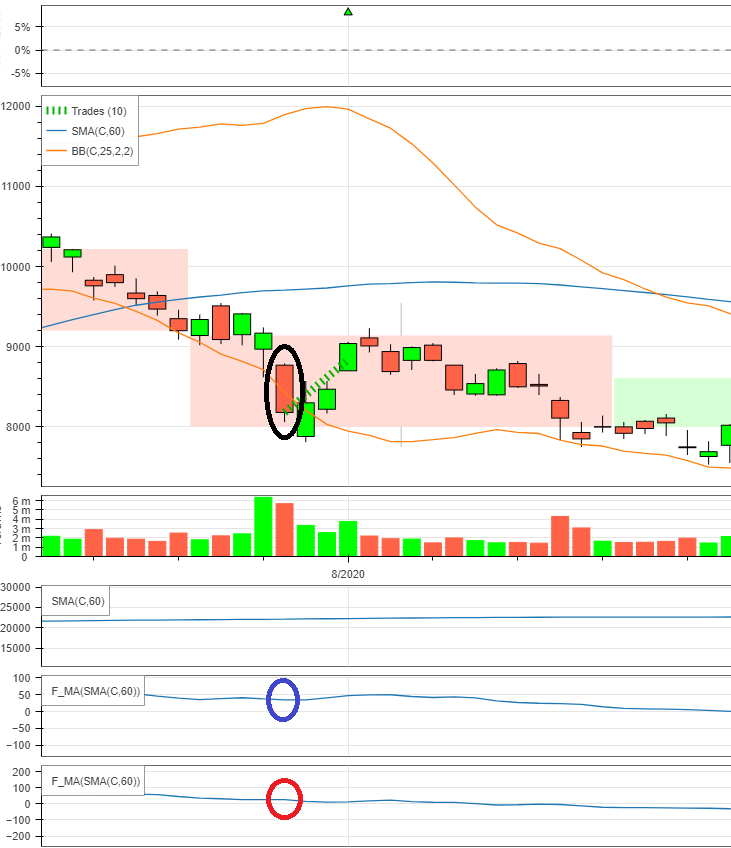
\includegraphics[width=110mm]{fig/bb_and_nk_and_fma_paint.png}
    \caption{(B9)アルゴリズムの買いシグナル}
    \label{fig:bbnkfma}
   \end{figure}

   


   \begin{figure}[H]
    \centering
    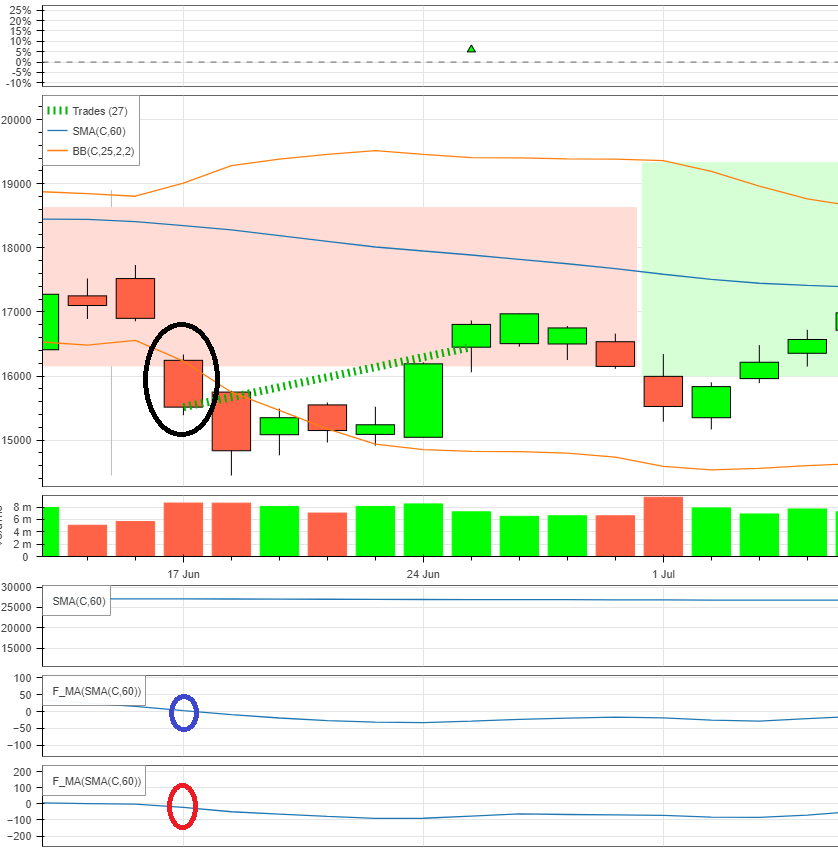
\includegraphics[width=110mm]{fig/bb_and_nk_or_fma0_paint.png}
    \caption{(B10)アルゴリズムの(1-1)と(1-2)の買いシグナル}
    \label{fig:bbnkfma0}
   \end{figure}

   \begin{figure}[H]
    \centering
    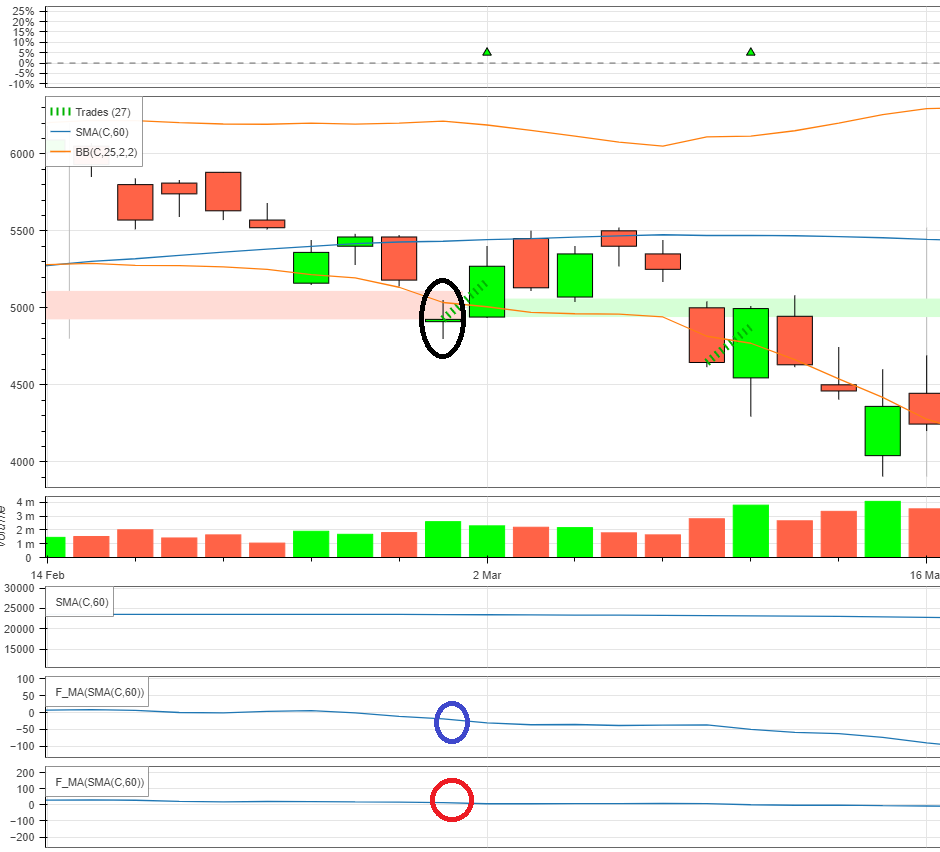
\includegraphics[width=110mm]{fig/bb_and_nk0_or_fma_paint.png}
    \caption{(B10)アルゴリズムの(1-1)と(1-3)の買いシグナル}
    \label{fig:bbnk0fma}
   \end{figure}
\begin{description}
  \item[\textbf{Step~1~:}]以下の(1-1)~(1-2)のどちらかの条件が満たされれば購入する.
  \begin{description}
    \item[\textbf{(1-1):}]MACDがシグナルを下から上へ突き抜けたときに翌日の始値で株を購入する.
    \item[\textbf{(1-2):}]注目する日のローソクの終値が-2σのBBを上から下へ突き抜けたときに終値で株を購入する.
   \end{description}  
  
  \item[\textbf{Step~2~:}]以下の(2-1)~(2-2)のどちらかの条件が満たされれば売却する.
   \begin{description}
    \item[\textbf{(2-1):}]株の始値が購入した株価より$tp$%以上になった時点で売る.
    \item[\textbf{(2-2):}]株の始値が購入した株価より$sl$%以下になった時点で売る. 
   \end{description}
  \item[\textbf{Step~3~:}]用意した株価データの最終日が来るまでStep 1からStep 3まで繰り返す.
  \end{description}
  


図\ref{fig:bb0macd},図\ref{fig:bbmacd0}にMACDとBよる買いシグナルの例を示す.図\ref{fig:bb0macd}の黒丸のBBはなにも起きていないが,赤丸がMACDの買いシグナルになっているので購入している.その後$tp$%以上で売っている.また,
図\ref{fig:bbmacd0}の赤丸のMACDはなにも起きていないが,黒丸がBBの買いシグナルになっているので購入している.その後$tp$%以上で売っている.
  %%%%%%%%%%%%%%%%
  \begin{figure}[H]
    \centering
    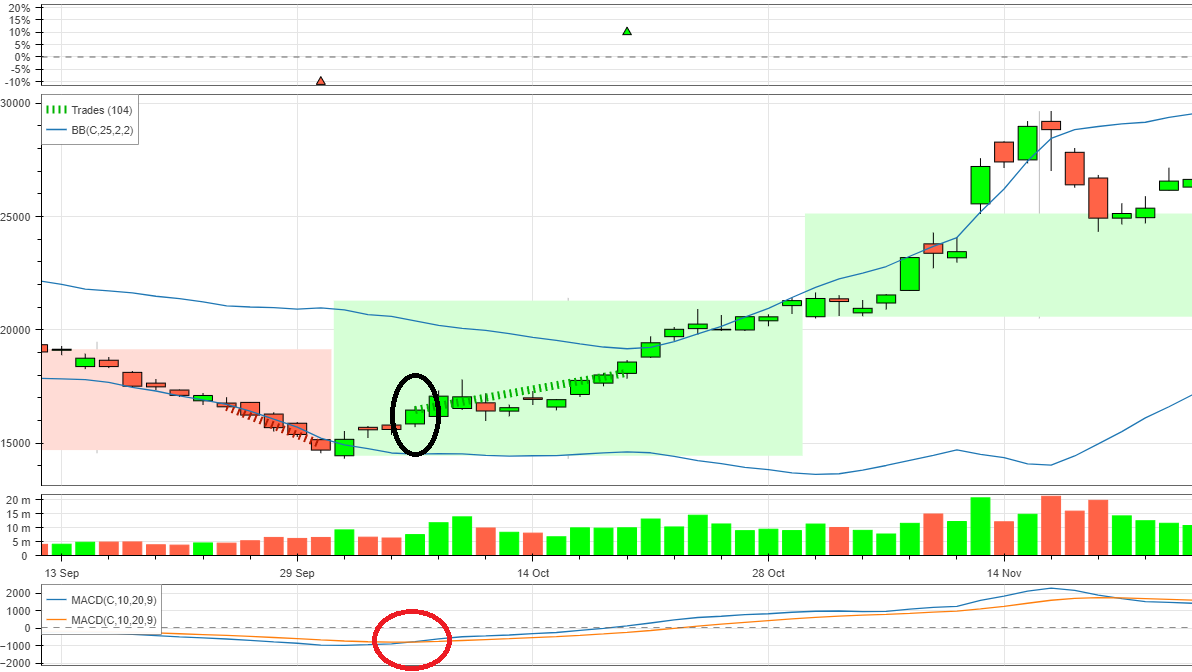
\includegraphics[width=110mm]{fig/bb0_or_macd_paint.png}
    \caption{(B11)アルゴリズムの(1-2)の買いシグナル}
    \label{fig:bb0macd}
   \end{figure}

  \begin{figure}[H]
    \centering
    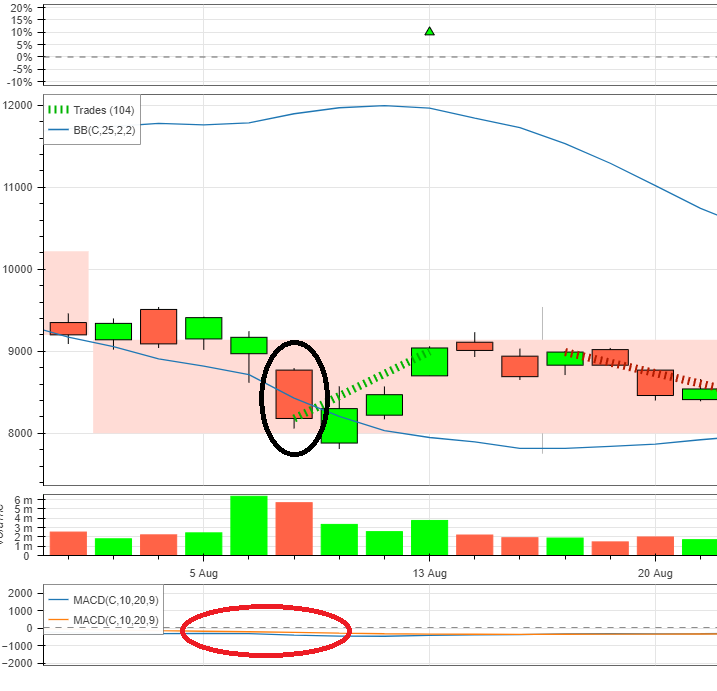
\includegraphics[width=110mm]{fig/bb_or_macd0_paint.png}
    \caption{(B11)アルゴリズムの(1-1)の買いシグナル}
    \label{fig:bbmacd0}
   \end{figure}
\subsection{MACDとBBと60日移動平均線}
MACDとBBと長期線を使う場合のトレーディングアルゴリズムを説明する.ここでは二通りの方法を説明する.(B11)に移動平均線を加えることで安定して勝率が上がるのではないかと想定している.ここでは最初に説明するアルゴリズムを(B12),その後に説明するアルゴリズムを(B13)とする.

   \begin{description}
    \item[\textbf{(B12):}]
    \item[\textbf{Step~1~:}]以下の(1-1)~(1-2)のどちらかと(1-3)の条件が満たされれば翌日購入するする.
    \begin{description}
      \item[\textbf{(1-1):}]注目する日のMACDがシグナルを下から上へ突き抜けたとき.
      \item[\textbf{(1-2):}]注目する日のローソクの終値が-2σのBBを上から下へ突き抜けたときに翌日の始値で株を購入する.
      \item[\textbf{(1-3):}]取引している株価データの長期線の傾きが0以上のとき. 
     \end{description}  
    
    
    \item[\textbf{Step~2~:}]以下の(2-1)~(2-2)のどちらかの条件が満たされれば売却する.
     \begin{description}
      \item[\textbf{(2-1):}]株の始値が購入した株価より$tp$%以上になった時点で売る.
      \item[\textbf{(2-2):}]株の始値が購入した株価より$sl$%以下になった時点で売る. 
     \end{description}
    \item[\textbf{Step~3~:}]用意した株価データの最終日が来るまでStep 1からStep 3まで繰り返す.
    \end{description}

    

     図\ref{fig:bb0ormacdfma},図\ref{fig:bbormacd0fma}にB12アルゴリズムの買いシグナルの例を示す.図\ref{fig:bb0ormacdfma}の青丸のBBはなにも起きていないが,黒丸がMACDの買いシグナルになっているのと,赤丸の長期線の傾きも0以上なので購入している.その後$tp$%以上で売っている.また,
     図\ref{fig:bbormacd0fma}の青丸のMACDはなにも起きていないが,黒丸がBBの買いシグナルになっているのと,赤丸の長期線の傾きも0以上なので購入している.その後$tp$%以上で売っている.
 
     \begin{description}
    \item[\textbf{(B13):}]
    \item[\textbf{Step~1~:}]以下の(1-1)の条件または(1-2),(1-3)のすべての条件が満たされれば翌日購入する.
    \begin{description}
      \item[\textbf{(1-1):}]注目する日のMACDがシグナルを下から上へ突き抜けたとき.
      \item[\textbf{(1-2):}]注目する日のローソクの終値が-2σのBBを上から下へ突き抜けたときに翌日の始値で株を購入する.
      \item[\textbf{(1-3):}]取引している株価データの長期線の傾きが0以上のとき. 

     \end{description}  
     \begin{figure}[H]
      \centering
      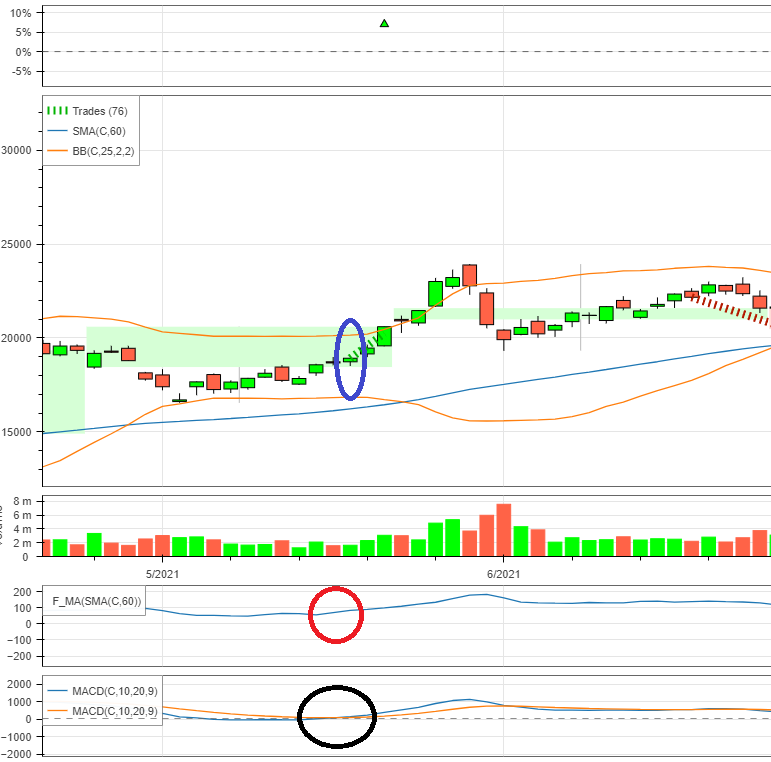
\includegraphics[width=110mm]{fig/macdorbb0_and_fma_paint.png}
      \caption{(B12)アルゴリズムの(1-1)と(1-3)の買いシグナル}
      \label{fig:bb0ormacdfma}
     \end{figure}
  
     \begin{figure}[H]
      \centering
      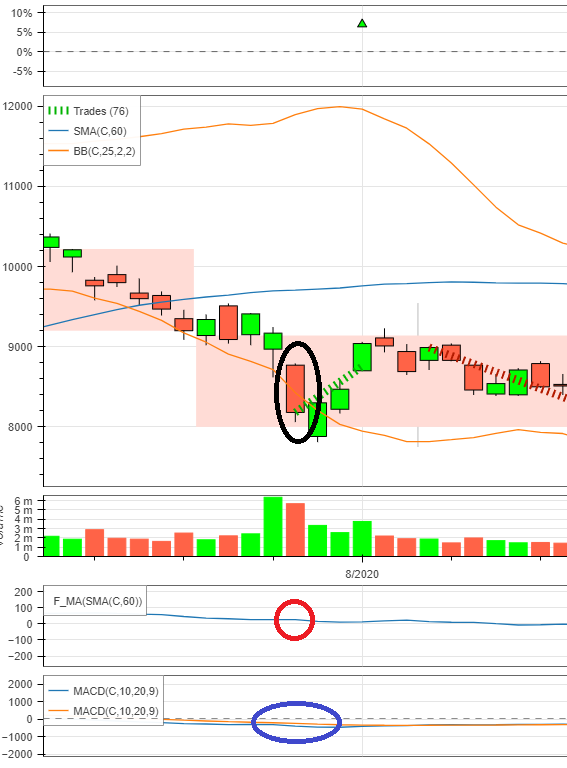
\includegraphics[width=110mm]{fig/macd0orbb_and_fma_paint.png}
      \caption{(B12)アルゴリズムの(1-2)と(1-3)の買いシグナル}
      \label{fig:bbormacd0fma}
     \end{figure}
    
    \item[\textbf{Step~2~:}]以下の(2-1)~(2-2)のどちらかの条件が満たされれば売却する.
     \begin{description}
      \item[\textbf{(2-1):}]株の始値が購入した株価より$tp$%以上になった時点で売る.
      \item[\textbf{(2-2):}]株の始値が購入した株価より$sl$%以下になった時点で売る. 
     \end{description}
    \item[\textbf{Step~3~:}]用意した株価データの最終日が来るまでStep 1からStep 3まで繰り返す.
    \end{description}

    
     図\ref{fig:bbfma0ormacd},図\ref{fig:bbfmaormacd0}に(B13)の買いシグナルの例を示す.図\ref{fig:bbfma0ormacd}の黒丸がMACDの買いシグナルになっているのと,赤丸の長期線の傾きも0以上だが青丸のBBはなにも起きていため,MACDの買いシグナルのみで購入している.その後$tp$%以上で売っている.また,
     図\ref{fig:bbfmaormacd0}の青丸のMACDはなにも起きていないが,黒丸がBBの買いシグナルになっているのと,赤丸の長期線の傾きも0以上なので購入している.その後$tp$%以上で売っている.







     
 

 




 


  



   

   \begin{figure}[H]
    \centering
    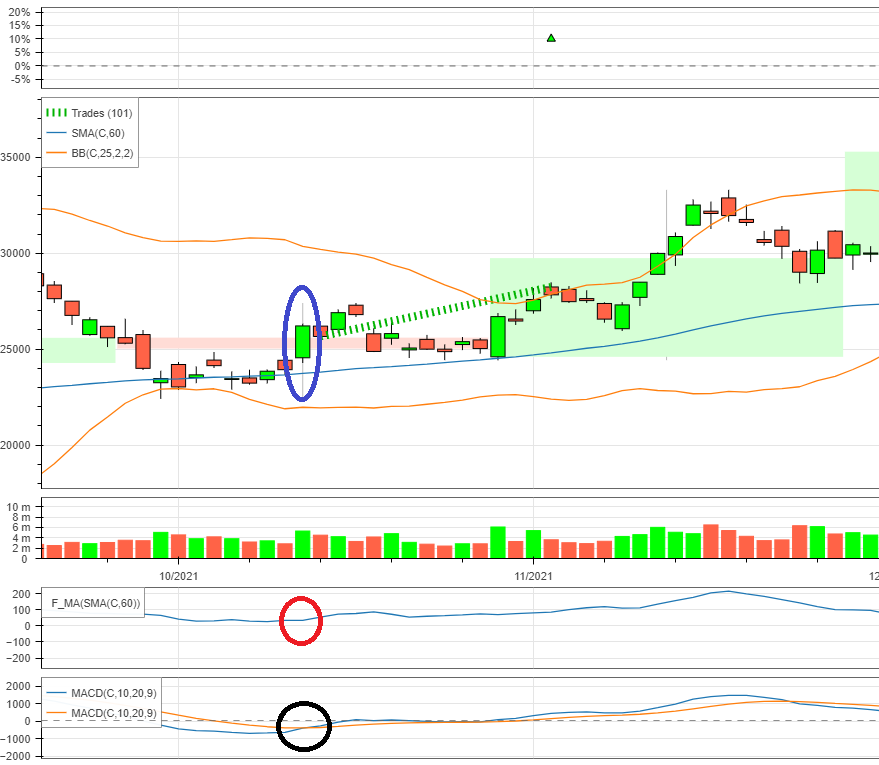
\includegraphics[width=110mm]{fig/bbandfma0_or_macd_paint.png}
    \caption{(B13)アルゴリズムの(1-1)の買いシグナル}
    \label{fig:bbfma0ormacd}
   \end{figure}

   \begin{figure}[H]
    \centering
    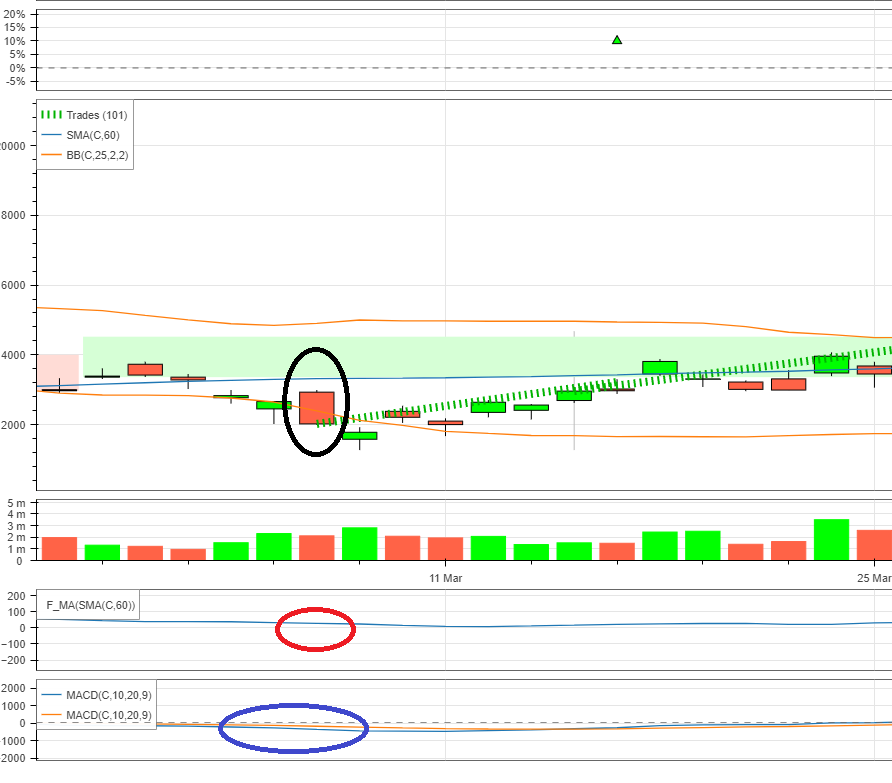
\includegraphics[width=110mm]{fig/bbandfma_or_macd0_paint.png}
    \caption{(B13)アルゴリズムの(1-2)と(1-3)の買いシグナル}
    \label{fig:bbfmaormacd0}
   \end{figure}
     \newpage
\chapter{実験結果}
本章では,前章で説明したトレーディングアルゴリズムを使って上位東証上位100社のうち2013年からのデータがある95株の
平均利益,平均勝率,最適化した平均$tp$,$ls$,平均トレード数を評価する.
\section{実験環境}
本研究における実験環境を表\ref{env}と\ref{lib}に表す.

\begin{table}[hbtp]
 \centering
 \caption{実験環境}
  \label{env}
 \begin{tabular}{|l||l|}
   \hline
   OS & Ubuntu 22.04.3 LTS\\
   \hline
   CPU & Intel Core i9-9900K\\
   \hline
   メモリ & 128GB \\
   \hline
   言語 & Python 3.10.12 \\
   \hline
  \end{tabular}
\end{table}

\begin{table}[hbtp]
  \centering
  \caption{ライブラリのバージョン}
   \label{lib}
  \begin{tabular}{|l||l|}
    \hline
    \textbf{ライブラリ} & \textbf{バージョン}\\
    \hline
    Backtesting & 0.3.3\\
    \hline
    ta-lib-bin & 0.4.26\\
    \hline
    numpy & 1.26.0 \\
    \hline
    pandas & 1.5.3 \\
    \hline
    matplotlib & 3.8.0 \\
    \hline
   \end{tabular}
 \end{table}
\newpage
\section{上位95社の株価データ}

検証で使った株価データのコードを表\ref{data}に表す.上位東証上位100社のうち2013年からのデータがある95株を使用する.

\begin{table}[htbp]
  \centering
  \caption{株コード}
  \label{data}
  \begin{tabular}{|l|l|l|l|l|}
  \hline
  \multicolumn{5}{|c|}{\textbf{株コード}} \\
  \hline
  
  1605 & 1925 & 1928 & 2502 & 2503 \\
  \hline
  2802 & 2914 & 3382 & 4063 & 4307 \\
  \hline
  4452 & 4502 & 4503 & 4507 & 4519 \\
  \hline
  4523 & 4543 & 4568 & 4578 & 4612 \\
  \hline
  4661 & 4684 & 4689 & 4901 & 4911 \\
  \hline
  5108 & 5401 & 6146 & 6201 & 6273 \\
  \hline
  6301 & 6326 & 6367 & 6501 & 6502 \\
  \hline
  6503 & 6594 & 6701 & 6702 & 6723 \\
  \hline
  6752 & 6758 & 6762 & 6857 & 6861 \\
  \hline
  6902 & 6920 & 6954 & 6971 & 6981 \\
  \hline
  7011 & 7201 & 7203 & 7267 & 7269 \\
  \hline
  7270 & 7532 & 7733 & 7741 & 7751 \\
  \hline
  7832 & 7974 & 8001 & 8002 & 8015 \\
  \hline
  8031 & 8035 & 8053 & 8058 & 8113 \\
  \hline
  8267 & 8306 & 8308 & 8309 & 8316 \\
  \hline
  8411 & 8591 & 8604 & 8630 & 8725 \\
  \hline
  8750 & 8766 & 8801 & 8802 & 9020 \\
  \hline
  9022 & 9101 & 9432 & 9433 & 9503 \\
  \hline
  9613 & 9735 & 9843 & 9983 & 9984 \\
  \hline
  \end{tabular}
\end{table}

これらの株価データの入手方法を以下に示す.
\begin{enumerate}
 \item まずはじめにhttps://finance.yahoo.comに行く.
 \item 次に検索バーに株コードを入れると候補欄が出てくるのでそこで選択する.
 \item 出てきたページのHistorical Dataを選択する.
 \item Time Periodの項目があるので選択して株価データの使う期間を選択する.本論文では2013年1月1日から2022年12月31日のデータを使う.
 \item Applyボタンがあるので押してその下にあるDownloadボタンを押せば,株価データのcsvファイルを取得することができる.
\end{enumerate}

\section{トレーディングアルゴリズムの検証}
第3章で説明した$tp$,$sl$を最適化してそれぞれのアルゴリズムを実行し,結果を以下の表\ref{strategy_comparison}に表す.$tp$,$sl$はそれぞれ101~110%,-99~-90%で最適化する.
図\ref{fig:res1}は,表\ref{strategy_comparison}の平均利益,平均取引数,平均勝率をグラフ化したもので,図\ref{fig:res2}は,表\ref{strategy_comparison}の平均TP,平均SLをグラフ化したものである.

また,図\ref{fig:macdonysai}から図\ref{fig:bbandfmmacdsai}までのグラフは,アルゴリズム(B1)から(B13)によって得られた95社の株の利益である.
\begin{table}[htbp]
  \small
  \centering
  \caption{各戦略の比較}
  \label{strategy_comparison}
  \begin{tabular}{|l||l|l|l|l|l|}
    \hline
    
  \textbf{戦略} & \textbf{平均利益} & \textbf{平均TP} & \textbf{平均SL} & \textbf{平均勝率\%} & \textbf{平均取引数} \\
  \hline

  (B1) & 212.02144 & 107.95789 & 93.48421 & 53.80\% & 67.32 \\\hline
  (B2) & 95.86136 & 107.47368 & 93.34737 & 56.36\% & 35.80 \\\hline
  (B3) & 80.29327 & 107.63158 & 93.29474 & 56.22\% & 34.51 \\\hline
  (B4) & 63.71441 & 107.52632 & 93.46316 & 57.08\% & 24.82 \\\hline
  (B5) & 122.89338 & 107.37895 & 93.35789 & 56.44\% & 45.95 \\\hline
  (B6) & 125.71012 & 107.68421 & 93.00000 & 58.99\% & 40.18 \\\hline
  (B7) & 57.27753 & 106.90526 & 92.76842 & 64.45\% & 19.48 \\\hline
  (B8) & 51.61579 & 106.50526 & 92.62105 & 67.32\% & 19.21 \\\hline
  (B9) & 39.39328 & 106.83158 & 93.27368 & 66.21\% & 12.36 \\\hline
  (B10) & 69.63080 & 106.66316 & 92.47368 & 64.45\% & 26.14 \\\hline
  (B11) & 305.81290 & 107.41053 & 93.57895 & 53.82\% & 98.56 \\\hline
  (B12) & 123.13827 & 107.14737 & 93.65263 & 56.25\% & 50.98 \\\hline
  (B13) & 238.55610 & 107.80000 & 93.57895 & 53.21\% & 78.83 \\\hline
 
  \end{tabular}
\end{table}

\begin{figure}[H]
  \centering
  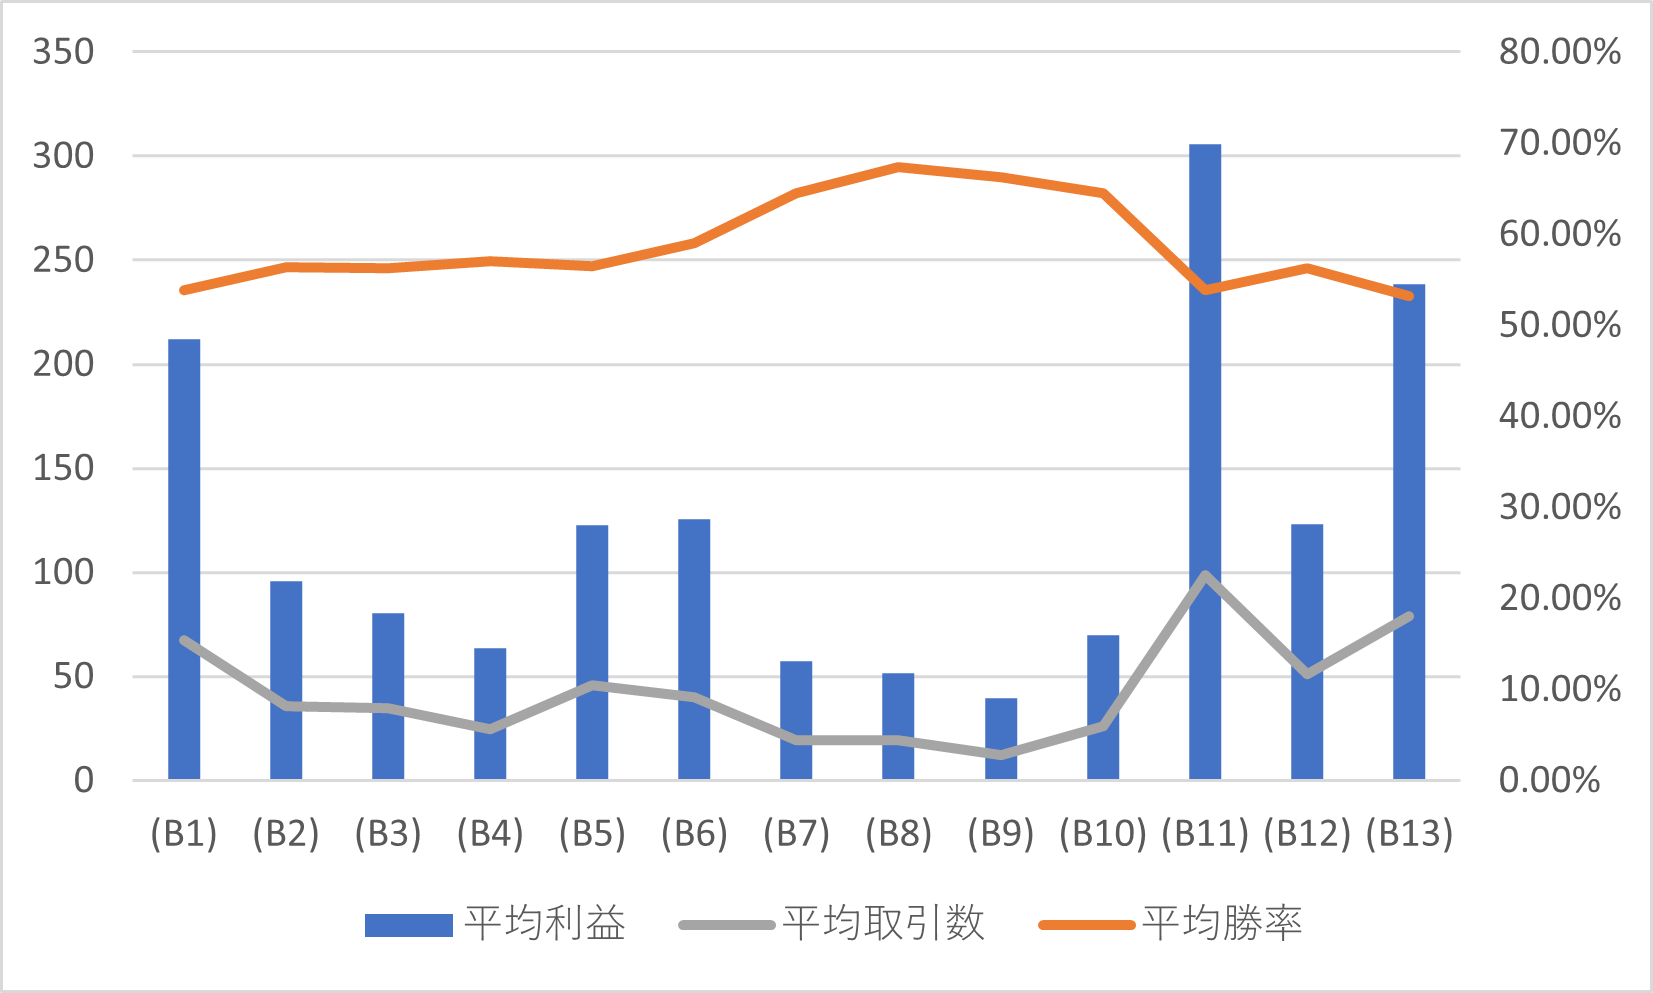
\includegraphics[width=110mm]{fig/res_1.png}
  \caption{平均利益,平均取引数,平均勝率のグラフ}
  \label{fig:res1}
 \end{figure}

 \begin{figure}[H]
  \centering
  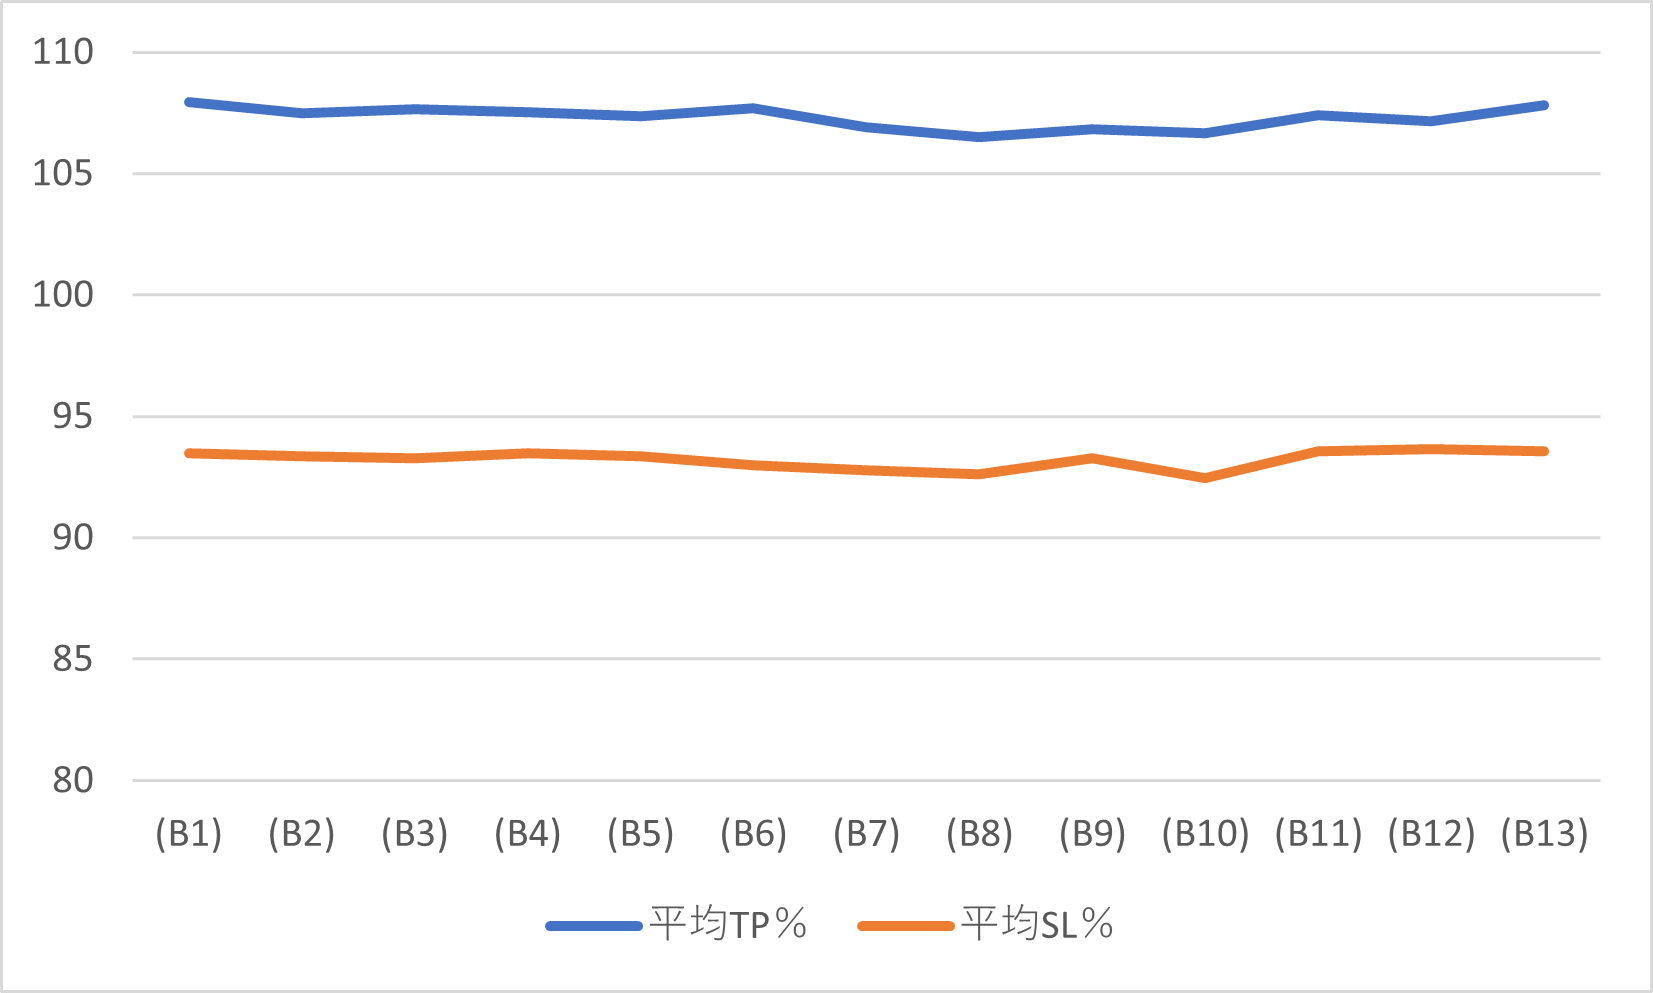
\includegraphics[width=110mm]{fig/res_2.png}
  \caption{平均SL,平均TPのグラフ}
  \label{fig:res2}
 \end{figure}

  \begin{figure}[H]
  \centering
  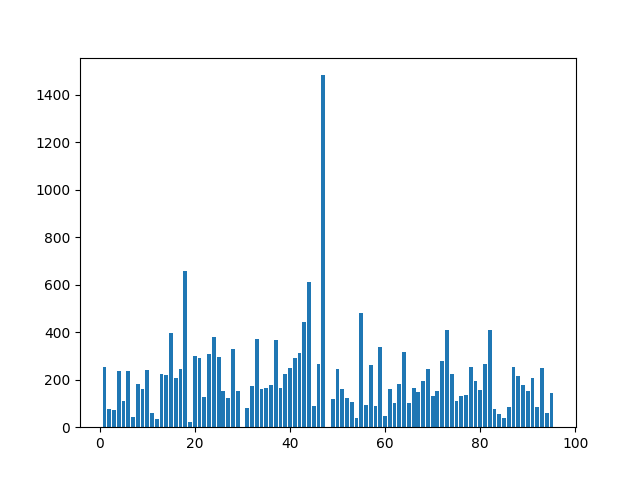
\includegraphics[width=110mm]{fig/macdonly_saiteki.png}
  \caption{アルゴリズムによる利益(B1)}
  \label{fig:macdonysai}
 \end{figure}

 \begin{figure}[H]
  \centering
  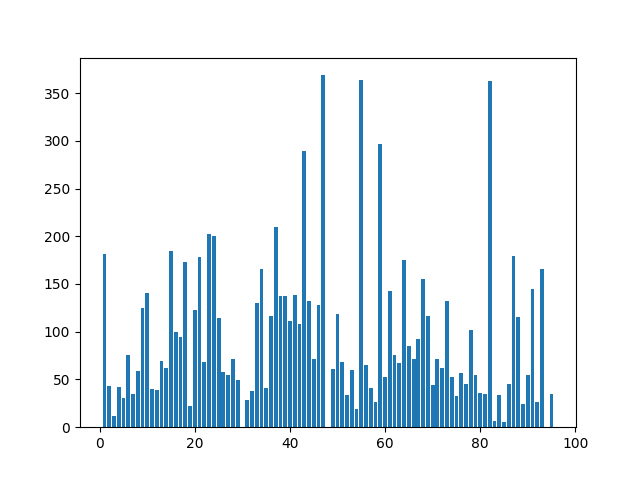
\includegraphics[width=110mm]{fig/macd_fma_saiteki.png}
  \caption{アルゴリズムによる利益(B2)}
  \label{fig:macdfmasai}
 \end{figure}

 \begin{figure}[H]
  \centering
  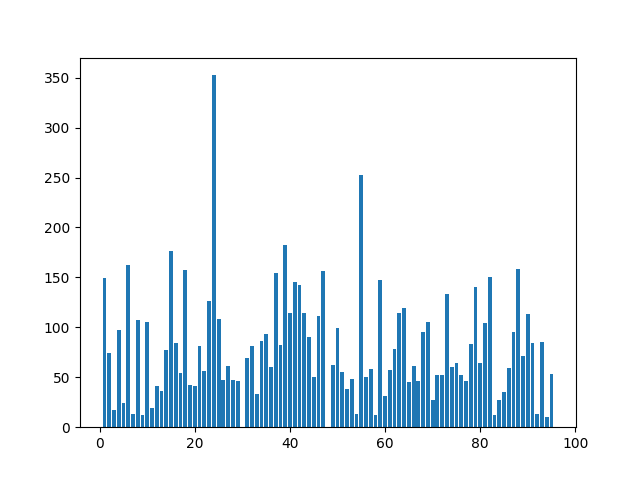
\includegraphics[width=110mm]{fig/macd_nikkei_saiteki.png}
  \caption{アルゴリズムによる利益(B3)}
  \label{fig:macdnikkeisai}
 \end{figure}

 \begin{figure}[H]
  \centering
  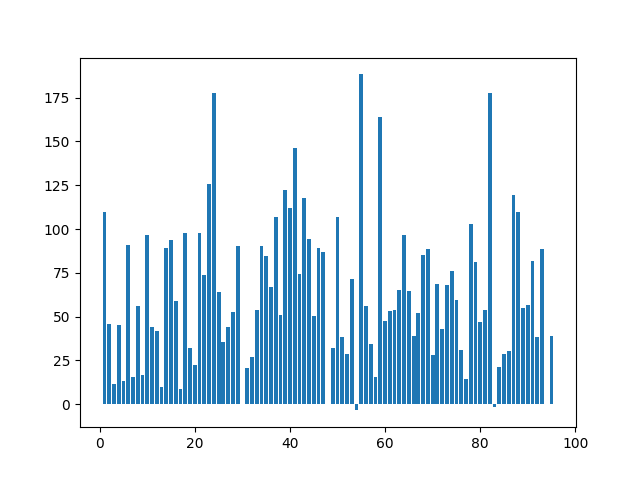
\includegraphics[width=110mm]{fig/macd_nikkeiandfma_saiteki.png}
  \caption{アルゴリズムによる利益(B4)}
  \label{fig:b4sai}
 \end{figure}

 \begin{figure}[H]
  \centering
  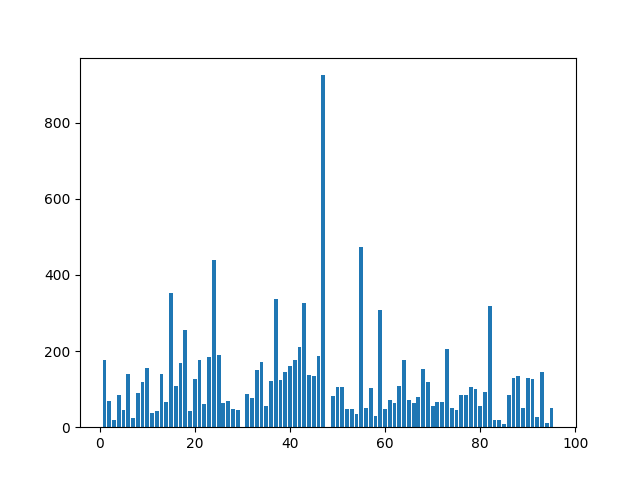
\includegraphics[width=110mm]{fig/macd_nikkeiorfma_saiteki.png}
  \caption{アルゴリズムによる利益(B5)}
  \label{fig:macdfmanksai}
 \end{figure}

 \begin{figure}[H]
  \centering
  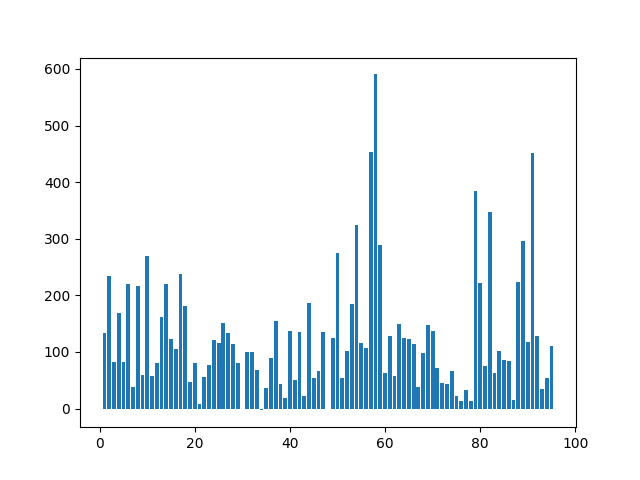
\includegraphics[width=110mm]{fig/bbonly_saiteki.png}
  \caption{アルゴリズムによる利益(B6)}
  \label{fig:bbsai}
 \end{figure}

 \begin{figure}[H]
  \centering
  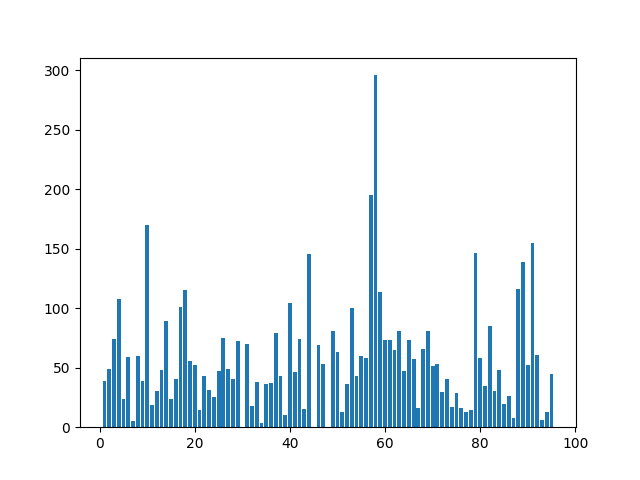
\includegraphics[width=110mm]{fig/bb_fma_saiteki.png}
  \caption{アルゴリズムによる利益(B7)}
  \label{fig:bbfmasai}
 \end{figure}

 \begin{figure}[H]
  \centering
  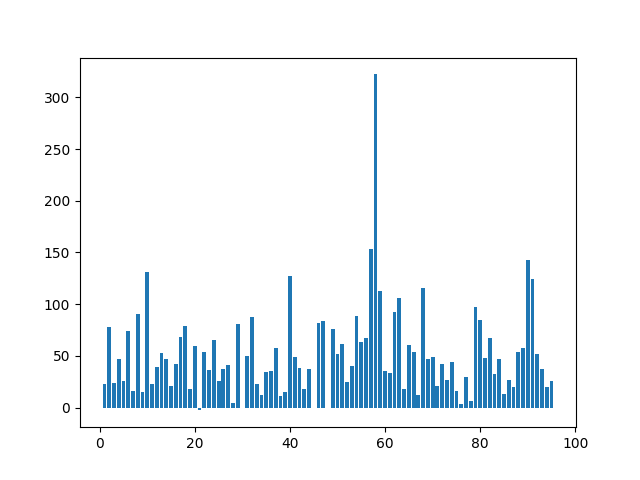
\includegraphics[width=110mm]{fig/bb_nikkei_saiteki.png}
  \caption{アルゴリズムによる利益(B8)}
  \label{fig:bbnikkeisai}
 \end{figure} 

 \begin{figure}[H]
  \centering
  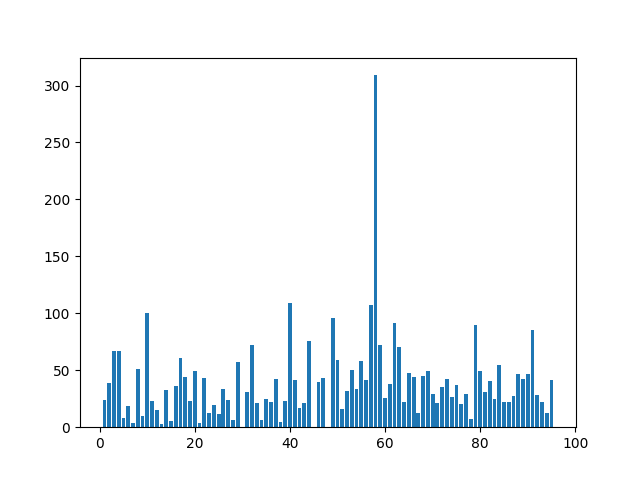
\includegraphics[width=110mm]{fig/bb_nikkeiandfma_saiteki.png}
  \caption{アルゴリズムによる利益(B9)}
  \label{fig:b9sai}
 \end{figure}

 \begin{figure}[H]
  \centering
  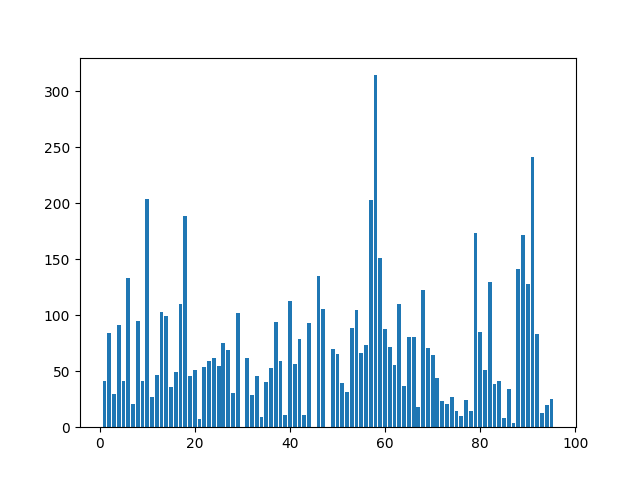
\includegraphics[width=110mm]{fig/bb_nikkeiorfma_saiteki.png}
  \caption{アルゴリズムによる利益(B10)}
  \label{fig:b10sai}
 \end{figure}

 \begin{figure}[H]
  \centering
  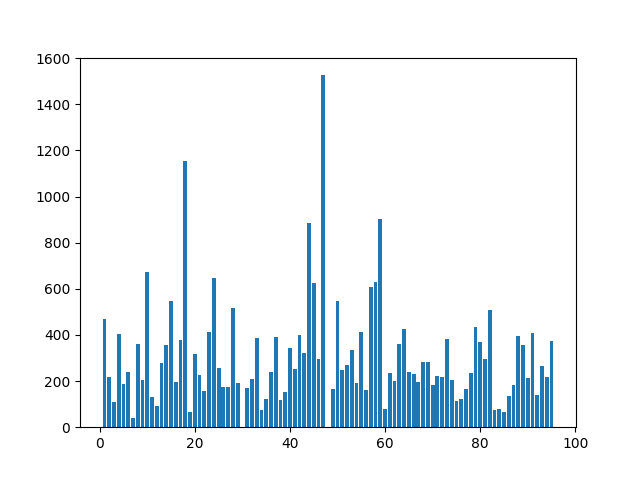
\includegraphics[width=110mm]{fig/bbmacdon_saiteki.png}
  \caption{アルゴリズムによる利益(B11)}
  \label{fig:bbmacdonsai}
 \end{figure}

 \begin{figure}[H]
  \centering
  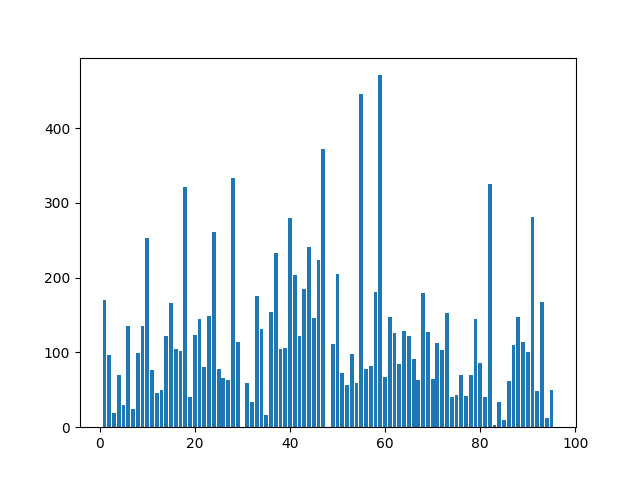
\includegraphics[width=110mm]{fig/bbmacdandfm_saiteki.png}
  \caption{アルゴリズムによる利益(B12)}
  \label{fig:bbmacdandfmsai}
 \end{figure}

 \begin{figure}[H]
  \centering
  \includegraphics[width=110mm]{fig/bbandfmmacd_saiteki.png}
  \caption{アルゴリズムによる利益(B13)}
  \label{fig:bbandfmmacdsai}
 \end{figure}

\section{実験結果と考察}

表\ref{strategy_comparison}より,利確に適している値は約107%で,損切りに適している値は約93%.
勝率は高くて67%,低くても53%であることがわかる.
また,利益が一番高いのは(B11)であることがわかる.これは
既存のよく使われている2つ指標を組み合わせているためだと考えられる.
BBとMACDそれぞれ同じ条件の場合だとMACDの利益が高くBBの勝率が高い.
(B9)の場合はすべてが同時になるという条件が厳しいため,利益と取引が一番低いが勝率が高くなりやすいことがわかる.

利益だけを追い求めるならばMACD主体のトレーディングアルゴリズムか(B11)を選択すればいいが,リスクが少ない方法を選びのならばBB主体のトレーディングアルゴリズム選択すればよいことがわかる.
\newpage
\chapter{まとめ}
本研究では,MACDとBBを用いていくつかのトレーディングアルゴリズムの提案を行った.既存のMACDとBBそれぞれ単体の場合よりも多い利益を出すことを示した.
また利益重視で取引するならばMACDを主体とした組み合わせ,利益と取引数は下がるが勝率重視で取引するならばBBを主体とした組み合わせのトレーディングアルゴリズムが良いことがわかった.
最大の利益を出したければ,利確を107%,損切りを93%にすれば良いという結果が得られた.

今後の課題として実際の取引でも使用されている他のテクニカル指標を用いたトレーディングアルゴリズムの提案と,AIを用いた場合の結果を比較することが挙げられる.
%% 参考文献


% 謝辞
\chapter*{謝辞}

\addcontentsline{toc}{chapter}{謝辞}
\markboth{}{謝辞}

\indent
本研究で知識不足な私に様々な助言を与えてくださった藤原暁宏教授に感謝します.また,ともに頑張ってきた同期のメンバーやわからないことなどにたいして
助言を与えてくださった,研究室の先輩に感謝します.株などの経済の知識を教えてくれて自分に興味を持たせてくれた従兄に感謝します.
最後に,何不自由なく大学で勉学に励めたのは,色々と助けてくれた両親のおかげです.心より感謝いたします.

%% 参考文献
%% アルファベット順(五十音順)
\newpage \addcontentsline{toc}{chapter}{\bibname}  % 「参考文献」を目次に表示
\bibliographystyle{jplain}
\begin{thebibliography}{99}
  \bibitem{morimoto}森本叡多郎,長期投資におけるトレーディングアルゴリズムの検証と提案,九州工業大学卒業論文,2022
  \bibitem{pythontrading}片渕彼富, “Pythonでできる!株価データの分析”,森北出版株式会社,2023
  %%
  \bibitem{pythonwhy}Python Software Foundation, What is Python? Executive Summary, \url{https://www.python.org/doc/essays/blurb/}
  %%
  \bibitem{pythonapp}Python Software Foundation, Applications for Python, \url{https://www.python.org/about/apps/}
  %%
  \bibitem{talib} TA-Lib - Technical Analysis Library,TA-Lib,\url{https://ta-lib.org/}
  %%
  \bibitem{finace}Yahoo!finace,Yahoo!finace, \url{https://finance.yahoo.com/}   
  %%
  \bibitem{datetime}Python Software Foundation,datetime --- 基本的な日付型および時間型,\url{https://docs.python.org/ja/3/library/datetime.html} 
  %%
  \bibitem{backtesting}github, backtesting.py ,\url{https://github.com/kernc/backtesting.py} 
  %%
  \bibitem{matplotlib}PyPI ,matplotlib 3.8.2,\url{https://pypi.org/project/matplotlib/}
  %%
  \bibitem{numpy}PyPI ,Numpy1.26.3,\url{https://pypi.org/project/numpy/}
  %%
  \bibitem{pandas}PyPI ,pandas 2.2.0,\url{https://pypi.org/project/pandas/}
  %%
  \bibitem{rikaku}日本取引所グループ,利益確定売り,\url{https://www.jpx.co.jp/glossary/ra/460.html}
  \bibitem{songiri}SMBC日興証券,損切り, \url{https://www.smbcnikko.co.jp/terms/japan/so/J0295.html}

  \bibitem{macdexp}QUICK Money World,MACDとは何か 見方や計算式,ゴールデンクロス・ダイバージェンスについても解説, \url{https://moneyworld.jp/news/05_00053723_news}
  \bibitem{stock}楽天証券,株とは,
  
  \url{https://www.rakuten-sec.co.jp/web/domestic/special/beginner/stock01.html}
  \bibitem{nikkei_kabu}SMBC日興証券,日経平均株価とは?,\url{https://www.smbc.co.jp/kojin/toushin/gimon/start12/}
  \bibitem{van}Vlogger,The History of Python,\url{https://python-history.blogspot.com/}
  \end{thebibliography}
  
%%%%%%%%%%%%%%%%%%%%%%%%%%%%%%%%%%%%%%%%%%%%%%
\appendix
\end{document}
